% Options for packages loaded elsewhere
\PassOptionsToPackage{unicode}{hyperref}
\PassOptionsToPackage{hyphens}{url}
%
\documentclass[
]{article}
\usepackage{amsmath,amssymb}
\usepackage{lmodern}
\usepackage[UTF8]{ctex}
\usepackage{ifxetex,ifluatex}
\ifnum 0\ifxetex 1\fi\ifluatex 1\fi=0 % if pdftex
  \usepackage[T1]{fontenc}
  \usepackage[utf8]{inputenc}
  \usepackage{textcomp} % provide euro and other symbols
\else % if luatex or xetex
  \usepackage{unicode-math}
  \defaultfontfeatures{Scale=MatchLowercase}
  \defaultfontfeatures[\rmfamily]{Ligatures=TeX,Scale=1}
\fi
% Use upquote if available, for straight quotes in verbatim environments
\IfFileExists{upquote.sty}{\usepackage{upquote}}{}
\IfFileExists{microtype.sty}{% use microtype if available
  \usepackage[]{microtype}
  \UseMicrotypeSet[protrusion]{basicmath} % disable protrusion for tt fonts
}{}
\makeatletter
\@ifundefined{KOMAClassName}{% if non-KOMA class
  \IfFileExists{parskip.sty}{%
    \usepackage{parskip}
  }{% else
    \setlength{\parindent}{0pt}
    \setlength{\parskip}{6pt plus 2pt minus 1pt}}
}{% if KOMA class
  \KOMAoptions{parskip=half}}
\makeatother
\usepackage{xcolor}
\IfFileExists{xurl.sty}{\usepackage{xurl}}{} % add URL line breaks if available
\IfFileExists{bookmark.sty}{\usepackage{bookmark}}{\usepackage{hyperref}}
\hypersetup{
  hidelinks,
  pdfcreator={LaTeX via pandoc}}
\urlstyle{same} % disable monospaced font for URLs
\usepackage{color}
\usepackage{fancyvrb}
\newcommand{\VerbBar}{|}
\newcommand{\VERB}{\Verb[commandchars=\\\{\}]}
\DefineVerbatimEnvironment{Highlighting}{Verbatim}{commandchars=\\\{\}}
% Add ',fontsize=\small' for more characters per line
\newenvironment{Shaded}{}{}
\newcommand{\AlertTok}[1]{\textcolor[rgb]{1.00,0.00,0.00}{\textbf{#1}}}
\newcommand{\AnnotationTok}[1]{\textcolor[rgb]{0.38,0.63,0.69}{\textbf{\textit{#1}}}}
\newcommand{\AttributeTok}[1]{\textcolor[rgb]{0.49,0.56,0.16}{#1}}
\newcommand{\BaseNTok}[1]{\textcolor[rgb]{0.25,0.63,0.44}{#1}}
\newcommand{\BuiltInTok}[1]{#1}
\newcommand{\CharTok}[1]{\textcolor[rgb]{0.25,0.44,0.63}{#1}}
\newcommand{\CommentTok}[1]{\textcolor[rgb]{0.38,0.63,0.69}{\textit{#1}}}
\newcommand{\CommentVarTok}[1]{\textcolor[rgb]{0.38,0.63,0.69}{\textbf{\textit{#1}}}}
\newcommand{\ConstantTok}[1]{\textcolor[rgb]{0.53,0.00,0.00}{#1}}
\newcommand{\ControlFlowTok}[1]{\textcolor[rgb]{0.00,0.44,0.13}{\textbf{#1}}}
\newcommand{\DataTypeTok}[1]{\textcolor[rgb]{0.56,0.13,0.00}{#1}}
\newcommand{\DecValTok}[1]{\textcolor[rgb]{0.25,0.63,0.44}{#1}}
\newcommand{\DocumentationTok}[1]{\textcolor[rgb]{0.73,0.13,0.13}{\textit{#1}}}
\newcommand{\ErrorTok}[1]{\textcolor[rgb]{1.00,0.00,0.00}{\textbf{#1}}}
\newcommand{\ExtensionTok}[1]{#1}
\newcommand{\FloatTok}[1]{\textcolor[rgb]{0.25,0.63,0.44}{#1}}
\newcommand{\FunctionTok}[1]{\textcolor[rgb]{0.02,0.16,0.49}{#1}}
\newcommand{\ImportTok}[1]{#1}
\newcommand{\InformationTok}[1]{\textcolor[rgb]{0.38,0.63,0.69}{\textbf{\textit{#1}}}}
\newcommand{\KeywordTok}[1]{\textcolor[rgb]{0.00,0.44,0.13}{\textbf{#1}}}
\newcommand{\NormalTok}[1]{#1}
\newcommand{\OperatorTok}[1]{\textcolor[rgb]{0.40,0.40,0.40}{#1}}
\newcommand{\OtherTok}[1]{\textcolor[rgb]{0.00,0.44,0.13}{#1}}
\newcommand{\PreprocessorTok}[1]{\textcolor[rgb]{0.74,0.48,0.00}{#1}}
\newcommand{\RegionMarkerTok}[1]{#1}
\newcommand{\SpecialCharTok}[1]{\textcolor[rgb]{0.25,0.44,0.63}{#1}}
\newcommand{\SpecialStringTok}[1]{\textcolor[rgb]{0.73,0.40,0.53}{#1}}
\newcommand{\StringTok}[1]{\textcolor[rgb]{0.25,0.44,0.63}{#1}}
\newcommand{\VariableTok}[1]{\textcolor[rgb]{0.10,0.09,0.49}{#1}}
\newcommand{\VerbatimStringTok}[1]{\textcolor[rgb]{0.25,0.44,0.63}{#1}}
\newcommand{\WarningTok}[1]{\textcolor[rgb]{0.38,0.63,0.69}{\textbf{\textit{#1}}}}
\usepackage{graphicx}
\makeatletter
\def\maxwidth{\ifdim\Gin@nat@width>\linewidth\linewidth\else\Gin@nat@width\fi}
\def\maxheight{\ifdim\Gin@nat@height>\textheight\textheight\else\Gin@nat@height\fi}
\makeatother
% Scale images if necessary, so that they will not overflow the page
% margins by default, and it is still possible to overwrite the defaults
% using explicit options in \includegraphics[width, height, ...]{}
\setkeys{Gin}{width=\maxwidth,height=\maxheight,keepaspectratio}
% Set default figure placement to htbp
\makeatletter
\def\fps@figure{htbp}
\makeatother
\setlength{\emergencystretch}{3em} % prevent overfull lines
\providecommand{\tightlist}{%
  \setlength{\itemsep}{0pt}\setlength{\parskip}{0pt}}
\setcounter{secnumdepth}{-\maxdimen} % remove section numbering
\ifluatex
  \usepackage{selnolig}  % disable illegal ligatures
\fi

\author{}
\date{}

\begin{document}

Java:
\href{https://medium.com/@krishankantsinghal/my-first-blog-on-medium-583159139237}{LRU
cache}

Python:
\href{https://docs.python.org/3/library/collections.html\#ordereddict-objects}{OrderDict}

\href{https://www.youtube.com/watch?v=qNRKPnOaUQE\&list=PLbaIOC0vpjNUg3b9zH14ikdknckN9hMMl}{经典考题}
1. calculator 2. number of islands

\hypertarget{dp-1-game-theory}{%
\subsection{\texorpdfstring{DP 1 game theory:
}{DP 1 game theory: }}\label{dp-1-game-theory}}

Stone Game I\textasciitilde IV

模版:

2player game 双方对称, 用dp计算先手玩家胜手数

\(dp[i] = sum(score[i:j]) - dp[j]\)

取i:j, 把交给对手, punish 对手的dp{[}j{]} (先后手反转,胜手数反转)

可使用prefix sum 或 suffix sum来优化sum

\begin{Shaded}
\begin{Highlighting}[]
\KeywordTok{def}\NormalTok{ Solution():}
  \KeywordTok{def}\NormalTok{ StoneGame(}\VariableTok{self}\NormalTok{, n, nums):}
    \CommentTok{\# recursive way}
    \KeywordTok{def}\NormalTok{ helper(n):}
      \AttributeTok{@lru\_cache}\NormalTok{(}\VariableTok{None}\NormalTok{)  }\CommentTok{\# auto memo in recursive call}
      \ControlFlowTok{if}\NormalTok{ n }\OperatorTok{\textless{}} \DecValTok{0}\NormalTok{: }\ControlFlowTok{return} \DecValTok{0}  \CommentTok{\# base case}
\NormalTok{      optimal }\OperatorTok{=} \BuiltInTok{float}\NormalTok{(}\StringTok{\textquotesingle{}inf\textquotesingle{}}\NormalTok{)  }\CommentTok{\# find optimal in DP formula}
      \ControlFlowTok{for}\NormalTok{ i }\KeywordTok{in}\NormalTok{ ...:}
\NormalTok{        optimal }\OperatorTok{=} \BuiltInTok{min}\NormalTok{(}\BuiltInTok{help}\NormalTok{(n}\OperatorTok{{-}}\NormalTok{i), optimal)  }\CommentTok{\# recursive call}
\NormalTok{      dp[i] }\OperatorTok{=}\NormalTok{ nums[i] }\OperatorTok{+}\NormalTok{ optimal}
			\ControlFlowTok{return}\NormalTok{ dp[i]}
   \ControlFlowTok{return}\NormalTok{ helper(n)}
		\CommentTok{\# iterative way 略}
\end{Highlighting}
\end{Shaded}

\hypertarget{dp-2}{%
\subsection{DP 2}\label{dp-2}}

\begin{Shaded}
\begin{Highlighting}[]
\CommentTok{\# kadane algo}
\NormalTok{init:}
\NormalTok{  max\_so\_far }\OperatorTok{=} \OperatorTok{{-}}\NormalTok{inf}
\NormalTok{ 	max\_ending\_here }\OperatorTok{=} \OperatorTok{{-}}\NormalTok{inf}
\ControlFlowTok{for}\NormalTok{ each i }\KeywordTok{in}\NormalTok{ a:}
\NormalTok{  max\_ending\_here }\OperatorTok{+=}\NormalTok{ a[i]}
\NormalTok{  max\_so\_far }\OperatorTok{=} \BuiltInTok{max}\NormalTok{(max\_so\_far, max\_ending\_here)}
\NormalTok{  max\_ending\_here }\OperatorTok{=} \BuiltInTok{max}\NormalTok{(max\_ending\_here, }\DecValTok{0}\NormalTok{)}
\ControlFlowTok{return}\NormalTok{ max\_so\_far}
\end{Highlighting}
\end{Shaded}

\hypertarget{dp-3-ux53ccux5e8fux5217}{%
\subsection{DP 3 双序列}\label{dp-3-ux53ccux5e8fux5217}}

1143 Longest Common Subsequence

\begin{Shaded}
\begin{Highlighting}[]
\NormalTok{f[i][j] }\OperatorTok{=}
\NormalTok{					when text1[i] }\OperatorTok{==}\NormalTok{ text2[j]		f[i}\OperatorTok{{-}}\DecValTok{1}\NormalTok{][j}\OperatorTok{{-}}\DecValTok{1}\NormalTok{]}
\NormalTok{  				otherwiese									}\BuiltInTok{max}\NormalTok{(f[i}\OperatorTok{{-}}\DecValTok{1}\NormalTok{][j], f[i][j}\OperatorTok{{-}}\DecValTok{1}\NormalTok{])}
\end{Highlighting}
\end{Shaded}

97 Interleaving String

\begin{Shaded}
\begin{Highlighting}[]
\NormalTok{f[i][j] }\OperatorTok{=}\NormalTok{  	f[i}\OperatorTok{{-}}\DecValTok{1}\NormalTok{][j] }\ControlFlowTok{if}\NormalTok{ 	s1[i}\OperatorTok{{-}}\DecValTok{1}\NormalTok{] }\OperatorTok{==}\NormalTok{ s3[i}\OperatorTok{+}\NormalTok{j}\OperatorTok{{-}}\DecValTok{1}\NormalTok{]}
\NormalTok{						f[i][j}\OperatorTok{{-}}\DecValTok{1}\NormalTok{] }\ControlFlowTok{if}\NormalTok{ 	s2[j}\OperatorTok{{-}}\DecValTok{1}\NormalTok{] }\OperatorTok{==}\NormalTok{ s3[i}\OperatorTok{+}\NormalTok{j}\OperatorTok{{-}}\DecValTok{1}\NormalTok{]}
\NormalTok{  					otherwise			}\VariableTok{False}
\end{Highlighting}
\end{Shaded}

72 Edit Distance (Converting word1 to word2, this operation is
sysmetric)

\begin{Shaded}
\begin{Highlighting}[]
\NormalTok{f[i][j] }\OperatorTok{=} \ControlFlowTok{if}\NormalTok{ word1[i}\OperatorTok{{-}}\DecValTok{1}\NormalTok{] }\OperatorTok{==}\NormalTok{ word2[j}\OperatorTok{{-}}\DecValTok{1}\NormalTok{]	dp[i][j] }\OperatorTok{=}\NormalTok{ dp[i}\OperatorTok{{-}}\DecValTok{1}\NormalTok{][j}\OperatorTok{{-}}\DecValTok{1}\NormalTok{]}
					\ControlFlowTok{else} 												\DecValTok{1} \OperatorTok{+} \BuiltInTok{min}\NormalTok{(dp[i}\OperatorTok{{-}}\DecValTok{1}\NormalTok{][j], dp[i][j}\OperatorTok{{-}}\DecValTok{1}\NormalTok{], dp[i}\OperatorTok{{-}}\DecValTok{1}\NormalTok{][j}\OperatorTok{{-}}\DecValTok{1}\NormalTok{])  }\CommentTok{\# 删, 增, 改}
\end{Highlighting}
\end{Shaded}

115 Distinct Subseq

\begin{Shaded}
\begin{Highlighting}[]
\NormalTok{f[i][j] }\OperatorTok{=} \CommentTok{\# direction don\textquotesingle{}t care}
\NormalTok{					f[i}\OperatorTok{{-}}\DecValTok{1}\NormalTok{][j}\OperatorTok{{-}}\DecValTok{1}\NormalTok{] }\OperatorTok{+}\NormalTok{ f[i}\OperatorTok{{-}}\DecValTok{1}\NormalTok{][j] when A[i] }\OperatorTok{==}\NormalTok{ B[j] (take)}
\NormalTok{  				f[i}\OperatorTok{{-}}\DecValTok{1}\NormalTok{][j] otherwise (skip) }
\end{Highlighting}
\end{Shaded}

10 Regular Expression ( . * no parenthesis)

\begin{Shaded}
\begin{Highlighting}[]
\NormalTok{f[string][pattern]}

\NormalTok{f[empty][empty] }\OperatorTok{=} \VariableTok{True}\OperatorTok{;}\NormalTok{ f[i][empty] }\OperatorTok{=} \VariableTok{False}\OperatorTok{;}\NormalTok{ pairs of zero}\OperatorTok{{-}}\NormalTok{matching }\OperatorTok{*}\NormalTok{ against empty string}
\ControlFlowTok{for}\NormalTok{ j }\KeywordTok{in}\NormalTok{ (}\DecValTok{2}\NormalTok{, }\BuiltInTok{len}\NormalTok{(pattern) }\OperatorTok{+} \DecValTok{1}\NormalTok{):  }\CommentTok{\# first char of pattern shouldn\textquotesingle{}t be *}
\NormalTok{  f[}\DecValTok{0}\NormalTok{][j] }\OperatorTok{=}\NormalTok{ f[}\DecValTok{0}\NormalTok{][j}\OperatorTok{{-}}\DecValTok{2}\NormalTok{] }\KeywordTok{and}\NormalTok{ pattern[j}\OperatorTok{{-}}\DecValTok{2}\NormalTok{] }\OperatorTok{==} \StringTok{\textquotesingle{}*\textquotesingle{}}
  \CommentTok{\# 				\^{} last pair of * gets us to empty string}
  \CommentTok{\#												\^{} this pair is a empty star pair}

\NormalTok{f[i][j] }\OperatorTok{=}   \CommentTok{\# we need to check B[j{-}1] if B[j] is *, transition is different when other direction}
\NormalTok{					when p[j] }\OperatorTok{==} \StringTok{\textquotesingle{}.\textquotesingle{}} \KeywordTok{or}\NormalTok{ s[i] }\OperatorTok{==}\NormalTok{ p[j]			f[i}\OperatorTok{{-}}\DecValTok{1}\NormalTok{][j}\OperatorTok{{-}}\DecValTok{1}\NormalTok{] }
\NormalTok{  				when p[j] }\OperatorTok{==} \StringTok{\textquotesingle{}*\textquotesingle{}}
\NormalTok{    												when p[j}\OperatorTok{{-}}\DecValTok{1}\NormalTok{] }\OperatorTok{=}\NormalTok{ s[i] 	f[i}\OperatorTok{{-}}\DecValTok{1}\NormalTok{][j] (consume one char)}
\NormalTok{      											otherwise						f[i][j}\OperatorTok{{-}}\DecValTok{2}\NormalTok{] (zero match star)}
\end{Highlighting}
\end{Shaded}

44 Wildcard Matching (? * wild-wild *)

\begin{Shaded}
\begin{Highlighting}[]
\NormalTok{f[string][pattern]}

\NormalTok{f[empty][empty] }\OperatorTok{=} \VariableTok{True}\OperatorTok{;}\NormalTok{ f[i][empty] }\OperatorTok{=} \VariableTok{False}\OperatorTok{;}\NormalTok{ pairs of zero}\OperatorTok{{-}}\NormalTok{matching }\OperatorTok{*}\NormalTok{ against empty string}
\ControlFlowTok{for}\NormalTok{ j }\KeywordTok{in}\NormalTok{ (}\DecValTok{1}\NormalTok{, }\BuiltInTok{len}\NormalTok{(pattern) }\OperatorTok{+} \DecValTok{1}\NormalTok{):  }\CommentTok{\# first char of pattern shouldn\textquotesingle{}t be *}
\NormalTok{  f[}\DecValTok{0}\NormalTok{][j] }\OperatorTok{=}\NormalTok{ f[}\DecValTok{0}\NormalTok{][j}\OperatorTok{{-}}\DecValTok{1}\NormalTok{] }\KeywordTok{and}\NormalTok{ pattern[j}\OperatorTok{{-}}\DecValTok{1}\NormalTok{] }\OperatorTok{==} \StringTok{\textquotesingle{}*\textquotesingle{}}
  \CommentTok{\# 				\^{} last pair of * gets us to empty string}
  \CommentTok{\#												\^{} this pair is a empty star pair}
\NormalTok{f[i][j] }\OperatorTok{=}
\NormalTok{					when p[j] }\OperatorTok{==} \StringTok{\textquotesingle{}?\textquotesingle{}} \KeywordTok{or}\NormalTok{ s[i] }\OperatorTok{==}\NormalTok{ p[j]			f[i}\OperatorTok{{-}}\DecValTok{1}\NormalTok{][j}\OperatorTok{{-}}\DecValTok{1}\NormalTok{] }
\NormalTok{  				when p[j] }\OperatorTok{==} \StringTok{\textquotesingle{}*\textquotesingle{}}\NormalTok{ 											f[i}\OperatorTok{{-}}\DecValTok{1}\NormalTok{][j] }\KeywordTok{or}\NormalTok{ f[i][j}\OperatorTok{{-}}\DecValTok{1}\NormalTok{]}

\end{Highlighting}
\end{Shaded}

1312 Min insertion to make a string palindrome

= len(s) - LCS(s, s.reverse())

516 Longest Palindromic Subsequence

= LCS(s, s.reverse())

1216 Valid Palindrome III

=

\hypertarget{dp-4-knapsack}{%
\subsection{\texorpdfstring{DP 4 Knapsack:
}{DP 4 Knapsack: }}\label{dp-4-knapsack}}

模版:

\begin{Shaded}
\begin{Highlighting}[]
\KeywordTok{def}\NormalTok{ knapsack():}
    \BuiltInTok{int}\NormalTok{ [N}\OperatorTok{+}\DecValTok{1}\NormalTok{][W}\OperatorTok{+}\DecValTok{1}\NormalTok{]}
\NormalTok{    dp[}\DecValTok{0}\NormalTok{][..] }\OperatorTok{=} \DecValTok{0}
\NormalTok{    dp[..][}\DecValTok{0}\NormalTok{] }\OperatorTok{=} \DecValTok{0}
    \ControlFlowTok{for}\NormalTok{ i }\KeywordTok{in}\NormalTok{ [}\FloatTok{1.}\NormalTok{.N]:}
    	\ControlFlowTok{for}\NormalTok{ w }\KeywordTok{in}\NormalTok{ [}\FloatTok{1.}\NormalTok{.W]:}
\NormalTok{    		dp[i][w] }\OperatorTok{=} \BuiltInTok{max}\NormalTok{(物品i放入, 物品i不放入)}
    \ControlFlowTok{return}\NormalTok{ dp[N][W]}
\end{Highlighting}
\end{Shaded}

\begin{Shaded}
\begin{Highlighting}[]
\CommentTok{// note that item list is unordered}
\CommentTok{// treat them independently: dp[j] means max value with j space left}
\CommentTok{// for each item, update dp[j] whose remaining space is valid }
\DataTypeTok{int}\NormalTok{ knapsack(}\DataTypeTok{int}\NormalTok{ val[], }\DataTypeTok{int}\NormalTok{ wt[], }\DataTypeTok{int}\NormalTok{ n, }\DataTypeTok{int}\NormalTok{ W)}
\NormalTok{\{}
    \DataTypeTok{int}\NormalTok{ dp[W+}\DecValTok{1}\NormalTok{];}
\NormalTok{    memset(dp, }\DecValTok{0}\NormalTok{, }\KeywordTok{sizeof}\NormalTok{(dp));}
    \ControlFlowTok{for}\NormalTok{(}\DataTypeTok{int}\NormalTok{ i=}\DecValTok{0}\NormalTok{; i \textless{} n; i++) }
        \ControlFlowTok{for}\NormalTok{(}\DataTypeTok{int}\NormalTok{ j=W; j\textgreater{}=wt[i]; j{-}{-})}
\NormalTok{            dp[j] = max(dp[j] , val[i] + dp[j{-}wt[i]]);  }\CommentTok{// dependence requires a reserved order }
    \ControlFlowTok{return}\NormalTok{ dp[W];}
\NormalTok{\}}
\end{Highlighting}
\end{Shaded}

\textbf{0-1 knapsack: solves \# of sub-arrays summing up to a value}

\begin{Shaded}
\begin{Highlighting}[]
\CommentTok{// find number of subset of an unordered list s.t. sum(subset) = target}
\KeywordTok{private} \DataTypeTok{int} \FunctionTok{subsetSum}\OperatorTok{(}\DataTypeTok{int}\OperatorTok{[]}\NormalTok{ nums}\OperatorTok{,} \DataTypeTok{int}\NormalTok{ S}\OperatorTok{)\{}
    \DataTypeTok{int}\OperatorTok{[]}\NormalTok{ dp }\OperatorTok{=} \KeywordTok{new} \DataTypeTok{int}\OperatorTok{[}\NormalTok{S}\OperatorTok{+}\DecValTok{1}\OperatorTok{];}
\NormalTok{    dp}\OperatorTok{[}\DecValTok{0}\OperatorTok{]} \OperatorTok{=} \DecValTok{1}\OperatorTok{;}
    \ControlFlowTok{for} \OperatorTok{(}\DataTypeTok{int}\NormalTok{ i }\OperatorTok{=} \DecValTok{0}\OperatorTok{;}\NormalTok{ i }\OperatorTok{\textless{}}\NormalTok{ nums}\OperatorTok{.}\FunctionTok{length}\OperatorTok{;}\NormalTok{ i}\OperatorTok{++)}
        \ControlFlowTok{for} \OperatorTok{(}\DataTypeTok{int}\NormalTok{ j }\OperatorTok{=}\NormalTok{ S}\OperatorTok{;}\NormalTok{ j }\OperatorTok{\textgreater{}=} \DecValTok{0}\OperatorTok{;}\NormalTok{ j}\OperatorTok{{-}{-})}
            \ControlFlowTok{if} \OperatorTok{(}\NormalTok{j }\OperatorTok{{-}}\NormalTok{ nums}\OperatorTok{[}\NormalTok{i}\OperatorTok{]} \OperatorTok{\textgreater{}=} \DecValTok{0}\OperatorTok{)}\NormalTok{ dp}\OperatorTok{[}\NormalTok{j}\OperatorTok{]} \OperatorTok{+=}\NormalTok{ dp}\OperatorTok{[}\NormalTok{j }\OperatorTok{{-}}\NormalTok{ nums}\OperatorTok{[}\NormalTok{i}\OperatorTok{]];}
    \ControlFlowTok{return}\NormalTok{ dp}\OperatorTok{[}\NormalTok{S}\OperatorTok{];}
\OperatorTok{\}}
\end{Highlighting}
\end{Shaded}

\begin{Shaded}
\begin{Highlighting}[]
\CommentTok{\# find number of subset of an unordered list s.t. sum(subset) = target}
\KeywordTok{def}\NormalTok{ subsetSum(nums, S):}
\NormalTok{    dp }\OperatorTok{=}\NormalTok{ [}\DecValTok{0}\NormalTok{] }\OperatorTok{*}\NormalTok{ (S}\OperatorTok{+}\DecValTok{1}\NormalTok{)  }\CommentTok{\# dp[i] is the max number of ways to reach i}
\NormalTok{    dp[}\DecValTok{0}\NormalTok{] }\OperatorTok{=} \DecValTok{1}
    \ControlFlowTok{for}\NormalTok{ n }\KeywordTok{in}\NormalTok{ nums:}
        \ControlFlowTok{for}\NormalTok{ j }\KeywordTok{in} \BuiltInTok{range}\NormalTok{(S }\OperatorTok{+} \DecValTok{1}\NormalTok{)[::}\OperatorTok{{-}}\DecValTok{1}\NormalTok{]:}
            \ControlFlowTok{if}\NormalTok{ j }\OperatorTok{{-}}\NormalTok{ n }\OperatorTok{\textgreater{}=} \DecValTok{0}\NormalTok{:}
\NormalTok{                dp[j] }\OperatorTok{+=}\NormalTok{ dp[j }\OperatorTok{{-}}\NormalTok{ n]  }\CommentTok{\# the new way to get sum of j is to include n; and there\textquotesingle{}re d[j {-} n] number of ways to do this}
    \ControlFlowTok{return}\NormalTok{ dp[}\OperatorTok{{-}}\DecValTok{1}\NormalTok{]}
\end{Highlighting}
\end{Shaded}

\hypertarget{dp-7-ux5750ux6807ux7c7b}{%
\subsection{DP 7 坐标类}\label{dp-7-ux5750ux6807ux7c7b}}

\href{https://leetcode.com/problems/partition-equal-subset-sum/}{416.
Partition Equal Subset Sum}

\href{https://leetcode.com/problems/ones-and-zeroes/}{474. Ones and
Zeroes}

\href{https://leetcode.com/problems/target-sum/}{494. Target Sum}

\hypertarget{binary-search-ux57faux7840ux7b97ux6cd5ii}{%
\subsection{Binary Search
基础算法II}\label{binary-search-ux57faux7840ux7b97ux6cd5ii}}

\(mid = left + (right - left) / 2\): avoid overflow

\begin{Shaded}
\begin{Highlighting}[]
\NormalTok{s }\OperatorTok{=} \DecValTok{0}
\NormalTok{e }\OperatorTok{=} \BuiltInTok{len} \OperatorTok{{-}} \DecValTok{1}
\ControlFlowTok{while}\NormalTok{(s }\OperatorTok{\textless{}=}\NormalTok{ e):}
\NormalTok{    mid }\OperatorTok{=}\NormalTok{ s }\OperatorTok{+}\NormalTok{ (e }\OperatorTok{{-}}\NormalTok{ s) }\OperatorTok{//} \DecValTok{2}
    \ControlFlowTok{if}\NormalTok{(nums[mid] }\OperatorTok{\textless{}}\NormalTok{ target):}
\NormalTok{        start }\OperatorTok{=}\NormalTok{ mid }\OperatorTok{+} \DecValTok{1}
    \ControlFlowTok{else}\NormalTok{:}
\NormalTok{        end }\OperatorTok{=}\NormalTok{ mid }\OperatorTok{{-}} \DecValTok{1}
\CommentTok{\# after termination end and start ptr are swapped, end = start {-} 1}
\end{Highlighting}
\end{Shaded}

\href{https://leetcode.com/problems/first-bad-version/}{278. First Bad
Version}

\href{https://leetcode.com/problems/median-of-two-sorted-arrays/}{4.
Median of Two Sorted Arrays} \textbf{HARD}

\href{https://leetcode.com/problems/split-array-largest-sum/}{410. Split
Array Largest Sum} \textbf{HARD} 二分法猜答案

\hypertarget{basic-calculator}{%
\subsection{\texorpdfstring{Basic Calculator
}{Basic Calculator }}\label{basic-calculator}}

\hypertarget{bfs}{%
\subsection{BFS}\label{bfs}}

\begin{Shaded}
\begin{Highlighting}[]
\KeywordTok{def}\NormalTok{ bfs(start: Node, target: Node) }\OperatorTok{{-}\textgreater{}} \BuiltInTok{int}\NormalTok{:}
\NormalTok{    q, visited, step }\OperatorTok{=}\NormalTok{ deque([start]), }\BuiltInTok{set}\NormalTok{([start]), }\DecValTok{0}
   	\ControlFlowTok{while}\NormalTok{ q:}
\NormalTok{        sz }\OperatorTok{=} \BuiltInTok{len}\NormalTok{(q)}
        \ControlFlowTok{for}\NormalTok{ i }\KeywordTok{in} \BuiltInTok{range}\NormalTok{(sz):}
\NormalTok{            cur }\OperatorTok{=}\NormalTok{ q.popleft()}
            \ControlFlowTok{if}\NormalTok{ cur }\OperatorTok{==}\NormalTok{ target:}
                \ControlFlowTok{return}\NormalTok{ step}
            \ControlFlowTok{for}\NormalTok{ x }\KeywordTok{in}\NormalTok{ cur.neighbor():}
                \ControlFlowTok{if} \KeywordTok{not}\NormalTok{ x }\KeywordTok{in}\NormalTok{ visited:}
\NormalTok{                    q.append(x)}
\NormalTok{                    visited.add(x)}
\NormalTok{         step }\OperatorTok{+=} \DecValTok{1}
\end{Highlighting}
\end{Shaded}

Bidirectional BFS in search graph:

\begin{Shaded}
\begin{Highlighting}[]
\KeywordTok{def}\NormalTok{ twoEndBfs(start: Node, target: Node) }\OperatorTok{{-}\textgreater{}} \BuiltInTok{int}\NormalTok{:}
\NormalTok{    beginQ, endQ, visited, step }\OperatorTok{=}\NormalTok{ deque([start]), deque([end]), }\BuiltInTok{set}\NormalTok{([start]), }\DecValTok{0}
    \ControlFlowTok{while}\NormalTok{ beginQ }\KeywordTok{and}\NormalTok{ endQ:}
\NormalTok{        nextQ }\OperatorTok{=}\NormalTok{ deque([])}
\NormalTok{        sz }\OperatorTok{=} \BuiltInTok{len}\NormalTok{(beginQ)}
        \ControlFlowTok{for}\NormalTok{ i }\KeywordTok{in} \BuiltInTok{range}\NormalTok{(sz):  }\CommentTok{\# 展开}
\NormalTok{            cur }\OperatorTok{=}\NormalTok{ beginQ.popleft()}
            \ControlFlowTok{for}\NormalTok{ x }\KeywordTok{in}\NormalTok{ cur.neighbor():}
                \ControlFlowTok{if}\NormalTok{ x }\KeywordTok{in}\NormalTok{ endQ:  }\CommentTok{\# endQ and startQ intersects}
                    \ControlFlowTok{return}\NormalTok{ step }\OperatorTok{+} \DecValTok{1}
                \ControlFlowTok{if} \KeywordTok{not}\NormalTok{ x }\KeywordTok{in}\NormalTok{ visited:}
\NormalTok{                    nextQ.append(x)}
        \ControlFlowTok{if} \BuiltInTok{len}\NormalTok{(endQ) }\OperatorTok{\textless{}} \BuiltInTok{len}\NormalTok{(nextQ):  }\CommentTok{\# performe reverse BFS from end if it\textquotesingle{}s better}
\NormalTok{        	beginQ }\OperatorTok{=}\NormalTok{ endQ}
\NormalTok{            endQ }\OperatorTok{=}\NormalTok{ nextQ}
        \ControlFlowTok{else}\NormalTok{:}
\NormalTok{            beginQ }\OperatorTok{=}\NormalTok{ endQ}
\NormalTok{        step }\OperatorTok{+=} \DecValTok{1}
    \ControlFlowTok{return} \DecValTok{0}
\end{Highlighting}
\end{Shaded}

Topological Sort:

\begin{Shaded}
\begin{Highlighting}[]
\KeywordTok{def}\NormalTok{ topologicalSort(graph dag):}
\NormalTok{    t }\OperatorTok{=}\NormalTok{ []  }\CommentTok{\# dag in topo order}
\NormalTok{    q, indegree }\OperatorTok{=}\NormalTok{ deque([]), }\BuiltInTok{dict}\NormalTok{()  }\CommentTok{\# stack, queue, whatever order}
    \ControlFlowTok{for}\NormalTok{ u, v }\KeywordTok{in}\NormalTok{ dag.edge():}
\NormalTok{    	indegree[v] }\OperatorTok{+=} \DecValTok{1}
\NormalTok{    q.add([i }\ControlFlowTok{for}\NormalTok{ i }\KeywordTok{in}\NormalTok{ indegree }\ControlFlowTok{if}\NormalTok{ indegree[i] }\OperatorTok{==} \DecValTok{0}\NormalTok{])}
    \ControlFlowTok{while}\NormalTok{ q:}
\NormalTok{        cur }\OperatorTok{=}\NormalTok{ q.popleft()}
        \ControlFlowTok{for}\NormalTok{ nei }\KeywordTok{in}\NormalTok{ cur.n eighbor():}
\NormalTok{            indegree[nei] }\OperatorTok{{-}=} \DecValTok{1}
            \ControlFlowTok{if}\NormalTok{ indegree[nei] }\OperatorTok{==} \DecValTok{0}\NormalTok{:}
\NormalTok{            	t.append(nei)}
	\ControlFlowTok{return}\NormalTok{ t  }\CommentTok{\# if len(t) != dag.vertex() then some cycle of isolated component exists}
\end{Highlighting}
\end{Shaded}

\$\$ graph representation adj list

\begin{Shaded}
\begin{Highlighting}[]
\CommentTok{\# adjcency list easy way}
\NormalTok{graph }\OperatorTok{=}\NormalTok{ defaultdict(}\BuiltInTok{list}\NormalTok{)  }\CommentTok{\# Map\textless{}Node, List\textless{}Node\textgreater{}\textgreater{}}
\ControlFlowTok{for}\NormalTok{ u, v }\KeywordTok{in}\NormalTok{ edge:}
\NormalTok{    graph[u].append(v)}
\CommentTok{\# adjcency list formal way}
\KeywordTok{class}\NormalTok{ AdjNode:}
    \KeywordTok{def} \FunctionTok{\_\_int\_\_}\NormalTok{(}\VariableTok{self}\NormalTok{, data):}
        \VariableTok{self}\NormalTok{.vertex }\OperatorTok{=}\NormalTok{ data}
        \VariableTok{self}\NormalTok{.}\BuiltInTok{next} \OperatorTok{=} \VariableTok{None}
\KeywordTok{class}\NormalTok{ Graph:}
    \KeywordTok{def} \FunctionTok{\_\_init\_\_}\NormalTok{(}\VariableTok{self}\NormalTok{, vertices):}
        \VariableTok{self}\NormalTok{.V }\OperatorTok{=}\NormalTok{ vertices}
        \VariableTok{self}\NormalTok{.graph }\OperatorTok{=}\NormalTok{ [}\VariableTok{None}\NormalTok{] }\OperatorTok{*} \VariableTok{self}\NormalTok{.V}
    \KeywordTok{def}\NormalTok{ add\_edge(}\VariableTok{self}\NormalTok{, src, dest):}
\NormalTok{        node }\OperatorTok{=}\NormalTok{ AdjNode(dest)}
\NormalTok{        node.}\BuiltInTok{next} \OperatorTok{=} \VariableTok{self}\NormalTok{.graph[src]}
        \VariableTok{self}\NormalTok{.graph[src] }\OperatorTok{=}\NormalTok{ node}
        \CommentTok{\#\# if undirected         }
        \CommentTok{\# node = AdjNode(src) }
        \CommentTok{\# node.next = self.graph[dest] }
        \CommentTok{\# self.graph[dest] = node }
\end{Highlighting}
\end{Shaded}

\hypertarget{back-tracing}{%
\subsection{back tracing}\label{back-tracing}}

\begin{Shaded}
\begin{Highlighting}[]
\CommentTok{\# backtracking}
\NormalTok{result }\OperatorTok{=}\NormalTok{ []}
\KeywordTok{def}\NormalTok{ bt(路径, 选择列表):}
    \ControlFlowTok{if}\NormalTok{ 满足条件:}
\NormalTok{        result.add(路径)}
        \ControlFlowTok{return}
   	\ControlFlowTok{for}\NormalTok{ 选项 }\KeywordTok{in}\NormalTok{ 选择列表:}
\NormalTok{        make}
\NormalTok{        bt(路径, 选项列表)}
\NormalTok{        unmake}
\end{Highlighting}
\end{Shaded}

tree traversal (iterative)

permuation I \& II, combination I \& II, subsets I \& II

\begin{Shaded}
\begin{Highlighting}[]
\CommentTok{\# human way of generating all subsets, }
\CommentTok{\# building from a empty set: }
\CommentTok{\# from left to right for each element, go to contain it }
\CommentTok{\# recursive call starting from the next position}
\CommentTok{\# go not contain it }
\KeywordTok{def}\NormalTok{ subsets(nums):}
\NormalTok{    n }\OperatorTok{=} \BuiltInTok{len}\NormalTok{(nums)}
\NormalTok{    res }\OperatorTok{=}\NormalTok{ []}
    \KeywordTok{def}\NormalTok{ bt(start, tmp):}
\NormalTok{        res.append(}\BuiltInTok{list}\NormalTok{(tmp))   }\CommentTok{\# res List[List[int]];}
        \ControlFlowTok{for}\NormalTok{ i }\KeywordTok{in} \BuiltInTok{range}\NormalTok{(start, n):}
\NormalTok{            tmp }\OperatorTok{+=}\NormalTok{ [nums[i]]}
\NormalTok{            bt(i }\OperatorTok{+} \DecValTok{1}\NormalTok{, tmp)}
\NormalTok{            tmp.pop()}
\NormalTok{    bt(}\DecValTok{0}\NormalTok{, [])}
    \ControlFlowTok{return}\NormalTok{ res}
\CommentTok{\# if duplicates exists, sort it and skip duplicated elements}
    \KeywordTok{def}\NormalTok{ subsetsWithDup(}\VariableTok{self}\NormalTok{, nums: List[}\BuiltInTok{int}\NormalTok{]) }\OperatorTok{{-}\textgreater{}}\NormalTok{ List[List[}\BuiltInTok{int}\NormalTok{]]:}
\NormalTok{        res }\OperatorTok{=}\NormalTok{ []}
\NormalTok{        nums }\OperatorTok{=} \BuiltInTok{sorted}\NormalTok{(nums)}
\NormalTok{        n }\OperatorTok{=} \BuiltInTok{len}\NormalTok{(nums)}
        \KeywordTok{def}\NormalTok{ bt(start, tmp):}
\NormalTok{            res.append(}\BuiltInTok{list}\NormalTok{(tmp))}
            \ControlFlowTok{for}\NormalTok{ i }\KeywordTok{in} \BuiltInTok{range}\NormalTok{(start, n):}
                \ControlFlowTok{if}\NormalTok{ i }\OperatorTok{!=}\NormalTok{ start }\KeywordTok{and}\NormalTok{ nums[i}\OperatorTok{{-}}\DecValTok{1}\NormalTok{] }\OperatorTok{==}\NormalTok{ nums[i]:}
                    \ControlFlowTok{continue}
\NormalTok{                tmp.append(nums[i])}
\NormalTok{                bt(i }\OperatorTok{+} \DecValTok{1}\NormalTok{, tmp)}
\NormalTok{                tmp.pop()}
\NormalTok{        bt(}\DecValTok{0}\NormalTok{, [])}
        \ControlFlowTok{return}\NormalTok{ res}
\end{Highlighting}
\end{Shaded}

\begin{Shaded}
\begin{Highlighting}[]
\CommentTok{\# similar way of bt, require that the len of array should be n}
\CommentTok{\# don\textquotesingle{}t choose an element if already included}
	\KeywordTok{def}\NormalTok{ permute(}\VariableTok{self}\NormalTok{, nums: List[}\BuiltInTok{int}\NormalTok{]) }\OperatorTok{{-}\textgreater{}}\NormalTok{ List[List[}\BuiltInTok{int}\NormalTok{]]:}
\NormalTok{        res }\OperatorTok{=}\NormalTok{ []}
\NormalTok{        n }\OperatorTok{=} \BuiltInTok{len}\NormalTok{(nums)}
        \KeywordTok{def}\NormalTok{ bt(tmp):}
            \ControlFlowTok{if} \BuiltInTok{len}\NormalTok{(tmp) }\OperatorTok{==}\NormalTok{ n:}
\NormalTok{                res.append(}\BuiltInTok{list}\NormalTok{(tmp))}
            \ControlFlowTok{for}\NormalTok{ i }\KeywordTok{in}\NormalTok{ nums:}
                \ControlFlowTok{if}\NormalTok{ i }\KeywordTok{in}\NormalTok{ tmp: }\ControlFlowTok{continue}
\NormalTok{                tmp.append(i)}
\NormalTok{                bt(tmp)}
\NormalTok{                tmp.pop()}
\NormalTok{        bt([])}
        \ControlFlowTok{return}\NormalTok{ res}
\CommentTok{\# if duplicate exsits? sort ! }
\CommentTok{\# if z appear more than once, use z\_1 then z\_2 then z\_3 }
\CommentTok{\# only add to list and call if z\_i{-}1 is used {-}{-}{-}\textgreater{}}
    \KeywordTok{def}\NormalTok{ permuteUnique(}\VariableTok{self}\NormalTok{, nums: List[}\BuiltInTok{int}\NormalTok{]) }\OperatorTok{{-}\textgreater{}}\NormalTok{ List[List[}\BuiltInTok{int}\NormalTok{]]:}
\NormalTok{        res }\OperatorTok{=}\NormalTok{ []}
\NormalTok{        n }\OperatorTok{=} \BuiltInTok{len}\NormalTok{(nums)}
\NormalTok{        nums }\OperatorTok{=} \BuiltInTok{sorted}\NormalTok{(nums)}
\NormalTok{        used\_ }\OperatorTok{=}\NormalTok{ [}\VariableTok{False} \ControlFlowTok{for}\NormalTok{ \_ }\KeywordTok{in} \BuiltInTok{range}\NormalTok{(n)]}
        \KeywordTok{def}\NormalTok{ bt(tmp, used):}
            \ControlFlowTok{if} \BuiltInTok{all}\NormalTok{(used):}
\NormalTok{                res.append(}\BuiltInTok{list}\NormalTok{(tmp))}
            \ControlFlowTok{for}\NormalTok{ i }\KeywordTok{in} \BuiltInTok{range}\NormalTok{(n):}
                \ControlFlowTok{if}\NormalTok{ used[i] }\KeywordTok{or}\NormalTok{ (i }\OperatorTok{!=} \DecValTok{0} \KeywordTok{and}\NormalTok{ nums[i}\OperatorTok{{-}}\DecValTok{1}\NormalTok{] }\OperatorTok{==}\NormalTok{ nums[i] }\KeywordTok{and} \KeywordTok{not}\NormalTok{ used[i}\OperatorTok{{-}}\DecValTok{1}\NormalTok{]):  }\CommentTok{\# \textless{}{-}{-}{-}}
                    \ControlFlowTok{continue}
\NormalTok{                used[i] }\OperatorTok{=} \VariableTok{True}
\NormalTok{                tmp.append(nums[i])}
\NormalTok{                bt(tmp, used)}
\NormalTok{                used[i] }\OperatorTok{=} \VariableTok{False}
\NormalTok{                tmp.pop()}
\NormalTok{        bt([], used\_)}
        \ControlFlowTok{return}\NormalTok{ res}
\CommentTok{\# combination, similar to permuation. only that require k elements instead}
    \KeywordTok{def}\NormalTok{ combine(}\VariableTok{self}\NormalTok{, n: }\BuiltInTok{int}\NormalTok{, k: }\BuiltInTok{int}\NormalTok{) }\OperatorTok{{-}\textgreater{}}\NormalTok{ List[List[}\BuiltInTok{int}\NormalTok{]]:}
\NormalTok{        res }\OperatorTok{=}\NormalTok{ []}
        \KeywordTok{def}\NormalTok{ bt(start, tmp):}
            \ControlFlowTok{if} \BuiltInTok{len}\NormalTok{(tmp) }\OperatorTok{==}\NormalTok{ k:}
\NormalTok{                res.append(}\BuiltInTok{list}\NormalTok{(tmp))}
                \ControlFlowTok{return}
            \ControlFlowTok{for}\NormalTok{ i }\KeywordTok{in} \BuiltInTok{range}\NormalTok{(start, n}\OperatorTok{+}\DecValTok{1}\NormalTok{):}
\NormalTok{                tmp.append(i)}
\NormalTok{                bt(i }\OperatorTok{+} \DecValTok{1}\NormalTok{, tmp)}
\NormalTok{                tmp.pop()}
\NormalTok{        bt(}\DecValTok{1}\NormalTok{, [])}
        \ControlFlowTok{return}\NormalTok{ res}
\end{Highlighting}
\end{Shaded}

Sudoku, NQueen

\begin{Shaded}
\begin{Highlighting}[]
\CommentTok{\# similar to sieve of eratosthenes}
\CommentTok{\# ban different location in a dfs run}
\KeywordTok{def}\NormalTok{ solveNQueens(}\VariableTok{self}\NormalTok{, n: }\BuiltInTok{int}\NormalTok{) }\OperatorTok{{-}\textgreater{}}\NormalTok{ List[List[}\BuiltInTok{str}\NormalTok{]]:}
\NormalTok{        res }\OperatorTok{=}\NormalTok{ []}
        \KeywordTok{def}\NormalTok{ dfs(queen: }\BuiltInTok{list}\NormalTok{, xy\_diff, xy\_sum):}
            \CommentTok{\# queen[i] is the 2nd{-}dim(y) location of the queen}
            \CommentTok{\# after putting a queen at (x, y), any location (i, j) s.t. i+j = x+y OR i{-}j = x{-}y OR j = y is banned}
\NormalTok{            x }\OperatorTok{=} \BuiltInTok{len}\NormalTok{(queen)}
            \ControlFlowTok{if}\NormalTok{ x }\OperatorTok{==}\NormalTok{ n:}
\NormalTok{                res.append(queen)}
                \ControlFlowTok{return}
            \ControlFlowTok{for}\NormalTok{ y }\KeywordTok{in} \BuiltInTok{range}\NormalTok{(n):}
                \ControlFlowTok{if}\NormalTok{ y }\KeywordTok{not} \KeywordTok{in}\NormalTok{ queen }\KeywordTok{and}\NormalTok{ x}\OperatorTok{+}\NormalTok{y }\KeywordTok{not} \KeywordTok{in}\NormalTok{ xy\_sum }\KeywordTok{and}\NormalTok{ x}\OperatorTok{{-}}\NormalTok{y }\KeywordTok{not} \KeywordTok{in}\NormalTok{ xy\_diff:}
                    \CommentTok{\# don\textquotesingle{}t backtrace, each dfs call is using a copy of the lists}
                    \CommentTok{\# if a thread failed to sovle, it just stops by not calling further dfs}
\NormalTok{                    dfs(queen }\OperatorTok{+}\NormalTok{ [y], xy\_diff }\OperatorTok{+}\NormalTok{ [x}\OperatorTok{{-}}\NormalTok{y], xy\_sum }\OperatorTok{+}\NormalTok{ [x}\OperatorTok{+}\NormalTok{y])}
\NormalTok{        res }\OperatorTok{=}\NormalTok{ []}
\NormalTok{        dfs([],[],[])}
\NormalTok{        retval }\OperatorTok{=}\NormalTok{ []}
        \CommentTok{\# output formatting, trivial }
        \ControlFlowTok{for}\NormalTok{ sol }\KeywordTok{in}\NormalTok{ res:}
\NormalTok{            tmp }\OperatorTok{=}\NormalTok{ []}
            \ControlFlowTok{for}\NormalTok{ y }\KeywordTok{in}\NormalTok{ sol:}
\NormalTok{                tmp.append(}\StringTok{\textquotesingle{}.\textquotesingle{}} \OperatorTok{*}\NormalTok{ y }\OperatorTok{+} \StringTok{\textquotesingle{}Q\textquotesingle{}} \OperatorTok{+} \StringTok{\textquotesingle{}.\textquotesingle{}} \OperatorTok{*}\NormalTok{ (n}\OperatorTok{{-}}\NormalTok{y}\OperatorTok{{-}}\DecValTok{1}\NormalTok{))}
\NormalTok{            retval.append(}\BuiltInTok{list}\NormalTok{(tmp))}
        \CommentTok{\# print(retval)}
        \ControlFlowTok{return}\NormalTok{ retval}
\end{Highlighting}
\end{Shaded}

\hypertarget{dfs}{%
\subsection{DFS}\label{dfs}}

binary tree traversal

\begin{Shaded}
\begin{Highlighting}[]
\KeywordTok{def}\NormalTok{ inorder(root):}
\NormalTok{  res, stack }\OperatorTok{=}\NormalTok{ [], []}
  \ControlFlowTok{while}\NormalTok{ root }\KeywordTok{and}\NormalTok{ stack:}
    \ControlFlowTok{while}\NormalTok{ root:}
\NormalTok{      stack.append(root)}
\NormalTok{      root }\OperatorTok{=}\NormalTok{ root.left}
   	\ControlFlowTok{if} \KeywordTok{not}\NormalTok{ stack:}
      \ControlFlowTok{return}\NormalTok{ res}
\NormalTok{   	node }\OperatorTok{=}\NormalTok{ stack.pop()}
\NormalTok{    res.append(node.val)}
\NormalTok{    root.node.right}
\KeywordTok{def}\NormalTok{ preorder(root):}
  \ControlFlowTok{if} \KeywordTok{not}\NormalTok{ root: }\ControlFlowTok{return}\NormalTok{ []}
\NormalTok{  res, stack }\OperatorTok{=}\NormalTok{ [], [root]}
  \ControlFlowTok{while}\NormalTok{ stack:}
\NormalTok{    node }\OperatorTok{=}\NormalTok{ stack.pop()}
\NormalTok{    res.append(node.val)}
    \ControlFlowTok{if}\NormalTok{ node.left:}
\NormalTok{      stack.append(node.left)}
    \ControlFlowTok{if}\NormalTok{ node.right:}
\NormalTok{      stack.append(node.right)}
\CommentTok{\textquotesingle{}\textquotesingle{}\textquotesingle{}def postorder(root):}
\CommentTok{  res, stack = [], []}
\CommentTok{  while True:}
\CommentTok{    while root:}
\CommentTok{      if root.right:}
\CommentTok{        stack.append(root.right)}
\CommentTok{      stack.append(root)}
\CommentTok{      root = root.left()\textquotesingle{}\textquotesingle{}\textquotesingle{}}
\end{Highlighting}
\end{Shaded}

\begin{Shaded}
\begin{Highlighting}[]
\CommentTok{\# \textbackslash{}remake }
\KeywordTok{def}\NormalTok{ preorder(root):}
\NormalTok{  res, stack }\OperatorTok{=}\NormalTok{ [], [root]}
  \ControlFlowTok{while}\NormalTok{ stack:}
\NormalTok{    root }\OperatorTok{=}\NormalTok{ stack.pop()}
\NormalTok{    res.append(root.val)}
    \ControlFlowTok{if}\NormalTok{ root.right: stack.append(root.right)}
    \ControlFlowTok{if}\NormalTok{ root.left:  stack.append(root.left)  }\CommentTok{\# stack, next pop will be left}
  \ControlFlowTok{return}\NormalTok{ res}

\KeywordTok{def}\NormalTok{ inorder(root):  }\CommentTok{\# inorder of BST is sorted ASC}
\NormalTok{  res, stack }\OperatorTok{=}\NormalTok{ [], []}
	\ControlFlowTok{while}\NormalTok{ root }\KeywordTok{or}\NormalTok{ stack:}
    \ControlFlowTok{while}\NormalTok{ root: }
\NormalTok{      stack.append(root.left)}
\NormalTok{      root }\OperatorTok{=}\NormalTok{ root.left}
\NormalTok{	root }\OperatorTok{=}\NormalTok{ stack.pop()}
\NormalTok{  res.appned(root.val)}
\NormalTok{  root }\OperatorTok{=}\NormalTok{ root.right}

\KeywordTok{def}\NormalTok{ postorder(root):  }
  \CommentTok{\# the post order is done by a reverse trick, following preorder way}
  \CommentTok{\# root, right, left ==rev==\textgreater{} left, right, root}
\NormalTok{  res, stack }\OperatorTok{=}\NormalTok{ deque([]), [root]}
  \ControlFlowTok{while}\NormalTok{ stack:}
\NormalTok{    root }\OperatorTok{=}\NormalTok{ stack.pop()}
\NormalTok{    res.appendleft(root.val)  }\CommentTok{\# always add to front}
    \ControlFlowTok{if}\NormalTok{ root.left: stack.append(root.left)}
    \ControlFlowTok{if}\NormalTok{ root.right: stack.append(root.right)}
  \ControlFlowTok{return}\NormalTok{ res}
\end{Highlighting}
\end{Shaded}

\href{https://www.lintcode.com/problem/nested-list-weight-sum/description}{Lint
\textbackslash551. Nested List Weight Sum}

\begin{Shaded}
\begin{Highlighting}[]
\CommentTok{"""}
\CommentTok{This is the interface that allows for creating nested lists.}
\CommentTok{You should not implement it, or speculate about its implementation}

\CommentTok{class NestedInteger(object):}
\CommentTok{    def isInteger(self):}
\CommentTok{        \# @return \{boolean\} True if this NestedInteger holds a single integer,}
\CommentTok{        \# rather than a nested list.}

\CommentTok{    def getInteger(self):}
\CommentTok{        \# @return \{int\} the single integer that this NestedInteger holds,}
\CommentTok{        \# if it holds a single integer}
\CommentTok{        \# Return None if this NestedInteger holds a nested list}

\CommentTok{    def getList(self):}
\CommentTok{        \# @return \{NestedInteger[]\} the nested list that this NestedInteger holds,}
\CommentTok{        \# if it holds a nested list}
\CommentTok{        \# Return None if this NestedInteger holds a single integer}
\CommentTok{"""}


\KeywordTok{class}\NormalTok{ Solution(}\BuiltInTok{object}\NormalTok{):}
    \CommentTok{\# @param \{NestedInteger[]\} nestedList a list of NestedInteger Object}
    \CommentTok{\# @return \{int\} an integer}
    \KeywordTok{def}\NormalTok{ depthSum(}\VariableTok{self}\NormalTok{, nestedList):}
        \CommentTok{\# Write your code here}
        \KeywordTok{def}\NormalTok{ dfs(nlist, depth) }\OperatorTok{{-}\textgreater{}} \BuiltInTok{int}\NormalTok{:}
            \ControlFlowTok{if} \KeywordTok{not}\NormalTok{ nlist:}
                \ControlFlowTok{return} \DecValTok{0}
\NormalTok{            res }\OperatorTok{=} \DecValTok{0}
            \ControlFlowTok{for}\NormalTok{ i }\KeywordTok{in}\NormalTok{ nlist:}
                \ControlFlowTok{if}\NormalTok{ i.isInteger():}
\NormalTok{                    res }\OperatorTok{+=}\NormalTok{ depth }\OperatorTok{*}\NormalTok{ i.getInteger()}
                \ControlFlowTok{else}\NormalTok{:}
\NormalTok{                    res }\OperatorTok{+=}\NormalTok{ dfs(i.getList(), depth}\OperatorTok{+}\DecValTok{1}\NormalTok{)}
            \ControlFlowTok{return}\NormalTok{ res}
        \ControlFlowTok{if} \KeywordTok{not}\NormalTok{ nestedList:}
            \ControlFlowTok{return} \DecValTok{0}
        \ControlFlowTok{return}\NormalTok{ dfs(nestedList, }\DecValTok{1}\NormalTok{)}
\end{Highlighting}
\end{Shaded}

\begin{Shaded}
\begin{Highlighting}[]
\KeywordTok{class}\NormalTok{ NestedIterator(}\BuiltInTok{object}\NormalTok{):}

    \KeywordTok{def} \FunctionTok{\_\_init\_\_}\NormalTok{(}\VariableTok{self}\NormalTok{, nestedList):}
        \CommentTok{"""}
\CommentTok{        Initialize your data structure here.}
\CommentTok{        :type nestedList: List[NestedInteger]}
\CommentTok{        """}
        \VariableTok{self}\NormalTok{.stack }\OperatorTok{=}\NormalTok{ nestedList[::}\OperatorTok{{-}}\DecValTok{1}\NormalTok{]}

    \KeywordTok{def} \BuiltInTok{next}\NormalTok{(}\VariableTok{self}\NormalTok{):}
        \CommentTok{"""}
\CommentTok{        :rtype: int}
\CommentTok{        """}
        \ControlFlowTok{return} \VariableTok{self}\NormalTok{.stack.pop().getInteger()}

    \KeywordTok{def}\NormalTok{ hasNext(}\VariableTok{self}\NormalTok{):}
        \CommentTok{"""}
\CommentTok{        :rtype: bool}
\CommentTok{        """}
        \ControlFlowTok{while} \VariableTok{self}\NormalTok{.stack:}
\NormalTok{            top }\OperatorTok{=} \VariableTok{self}\NormalTok{.stack[}\OperatorTok{{-}}\DecValTok{1}\NormalTok{]}
            \ControlFlowTok{if}\NormalTok{ top.isInteger():}
                \ControlFlowTok{return} \VariableTok{True}
            \VariableTok{self}\NormalTok{.stack }\OperatorTok{=} \VariableTok{self}\NormalTok{.stack[:}\OperatorTok{{-}}\DecValTok{1}\NormalTok{] }\OperatorTok{+}\NormalTok{ top.getList()[::}\OperatorTok{{-}}\DecValTok{1}\NormalTok{]}
        \ControlFlowTok{return} \VariableTok{False}
\end{Highlighting}
\end{Shaded}

\href{https://www.lintcode.com/problem/inorder-successor-in-bst/discuss}{\textbackslash448.
Inorder Successor in BST}

\begin{Shaded}
\begin{Highlighting}[]
\KeywordTok{def}\NormalTok{ inorderSuccessor(}\VariableTok{self}\NormalTok{, root, p):}
        \CommentTok{\# write your code here}
        \CommentTok{\# O(n) Ignore BST property:}
        \CommentTok{\# keep a prev ptr to keep track of p, then we can search of node whose\textquotesingle{}s prev is p}
        \CommentTok{\# by inorder traversal}
\NormalTok{        curr, prev, stack }\OperatorTok{=}\NormalTok{ root, }\VariableTok{None}\NormalTok{, []}
        \ControlFlowTok{while}\NormalTok{ curr }\KeywordTok{or}\NormalTok{ stack:}
            \ControlFlowTok{while}\NormalTok{ curr:}
\NormalTok{                stack.append(curr)}
\NormalTok{                curr }\OperatorTok{=}\NormalTok{ curr.left }
            \CommentTok{\# curr = None}
\NormalTok{            curr }\OperatorTok{=}\NormalTok{ stack.pop()}
            \ControlFlowTok{if}\NormalTok{ prev }\KeywordTok{and}\NormalTok{ prev.val }\OperatorTok{==}\NormalTok{ p.val:}
                \ControlFlowTok{return}\NormalTok{ curr}
\NormalTok{            prev }\OperatorTok{=}\NormalTok{ curr}
\NormalTok{            curr }\OperatorTok{=}\NormalTok{ curr.right}
        \ControlFlowTok{return} \VariableTok{None}
        \CommentTok{\# O(h) }
        \KeywordTok{def}\NormalTok{ findmin(p):}
            \ControlFlowTok{while}\NormalTok{ p.left:}
\NormalTok{                p }\OperatorTok{=}\NormalTok{ p.left}
            \ControlFlowTok{return}\NormalTok{ p}
        \ControlFlowTok{if} \KeywordTok{not}\NormalTok{ root }\KeywordTok{or} \KeywordTok{not}\NormalTok{ p: }\ControlFlowTok{return} \VariableTok{None}
        \ControlFlowTok{if}\NormalTok{ p.right:}
            \ControlFlowTok{return}\NormalTok{ findmin(p.right)}
        \ControlFlowTok{else}\NormalTok{:}
\NormalTok{            ans }\OperatorTok{=} \VariableTok{None}
            \ControlFlowTok{while}\NormalTok{ root:}
                \ControlFlowTok{if}\NormalTok{ p.val }\OperatorTok{==}\NormalTok{ root.val:}
                    \ControlFlowTok{return}\NormalTok{ ans}
                \ControlFlowTok{if}\NormalTok{ p.val }\OperatorTok{\textgreater{}}\NormalTok{ root.val:}
\NormalTok{                    root }\OperatorTok{=}\NormalTok{ root.right}
                \ControlFlowTok{else}\NormalTok{:}
\NormalTok{                    ans }\OperatorTok{=}\NormalTok{ root}
\NormalTok{                    root }\OperatorTok{=}\NormalTok{ root.left}
            \ControlFlowTok{return} \VariableTok{None}
\end{Highlighting}
\end{Shaded}

\hypertarget{sliding-windows}{%
\subsection{Sliding Windows}\label{sliding-windows}}

\href{https://www.lintcode.com/problem/longest-substring-with-at-most-k-distinct-characters/description}{386.
Longest Substring with At Most K Distinct Characters}

\begin{Shaded}
\begin{Highlighting}[]
\KeywordTok{def}\NormalTok{ lengthOfLongestSubstringKDistinct(s: }\BuiltInTok{str}\NormalTok{, k: }\BuiltInTok{int}\NormalTok{) }\OperatorTok{{-}\textgreater{}} \BuiltInTok{int}\NormalTok{:}
  \KeywordTok{def}\NormalTok{ invalid(hashmap, k):}
    \CommentTok{\# valid or invalid, determine if hashmap defines a valid window}
    \CommentTok{\# valid: trim left to find a smallest window that is still valid}
    \CommentTok{\# invalid: trim left to find a largest sub{-}window that is valid }
    \CommentTok{\# Valid Ex: len(hashmap.keys()) == k; each all(haspmap.values() \textgreater{}= k); etc }
    \ControlFlowTok{return} \BuiltInTok{len}\NormalTok{(hashmap) }\OperatorTok{\textgreater{}}\NormalTok{ k}
\NormalTok{  hashmap }\OperatorTok{=} \BuiltInTok{dict}\NormalTok{()}
\NormalTok{  left, res }\OperatorTok{=} \DecValTok{0}\NormalTok{, }\DecValTok{0}
  \ControlFlowTok{for}\NormalTok{ i }\KeywordTok{in} \BuiltInTok{range}\NormalTok{(}\BuiltInTok{len}\NormalTok{(s)):  }
    \CommentTok{\# \textless{}{-} record the result here \textquotesingle{}while valid trim to minimize\textquotesingle{}}
\NormalTok{    c }\OperatorTok{=}\NormalTok{ s[i]}
    \ControlFlowTok{if}\NormalTok{ c }\KeywordTok{in}\NormalTok{ hashmap: hashmap[c] }\OperatorTok{+=} \DecValTok{1}
    \ControlFlowTok{else}\NormalTok{: hashmap[c] }\OperatorTok{=} \DecValTok{1}
    \ControlFlowTok{while}\NormalTok{ invalid(hashmap, k):}
\NormalTok{      left\_c }\OperatorTok{=}\NormalTok{ s[left]}
\NormalTok{      hashmap[left\_c] }\OperatorTok{{-}=} \DecValTok{1}
      \ControlFlowTok{if}\NormalTok{ hashmap[left\_c] }\OperatorTok{==} \DecValTok{0}\NormalTok{:}
        \KeywordTok{del}\NormalTok{ hashmap[left\_c]}
\NormalTok{      left }\OperatorTok{+=} \DecValTok{1}
\NormalTok{    res }\OperatorTok{=} \BuiltInTok{max}\NormalTok{(res, i }\OperatorTok{{-}}\NormalTok{ left }\OperatorTok{+} \DecValTok{1}\NormalTok{)  }\CommentTok{\# \textless{}{-} record the result here \textquotesingle{}while invalid trim\textquotesingle{}}
  \ControlFlowTok{return}\NormalTok{ res}
\end{Highlighting}
\end{Shaded}

\begin{enumerate}
\def\labelenumi{\arabic{enumi}.}
\item
  exact K -\textgreater{} atMost(K) - atMost(K-1), handles duplicates
  well
\item
  字母类可以尝试枚举 \# of distinct = 1, 2, 3, ...., 26
\item
  hard 考虑 单调队列 (unseen)
\end{enumerate}

\hypertarget{catches}{%
\subsection{Catches}\label{catches}}

if two string has the same length -\textgreater{} sum of Counter is the
same. If the Counter is different, then some element must be negative.
242

a string with n pair of balanced parentheses: as we add new char into
the str, \#(lp) is always \textless{} n AND \#(rp) is always \textless{}
\#(lp)

KMP is a plus

\href{https://www.geeksforgeeks.org/sort-an-array-of-0s-1s-and-2s/}{Dutch
National Flag Algo} 75

\begin{Shaded}
\begin{Highlighting}[]
\CommentTok{\# eratosthenes prime finding}
\KeywordTok{def}\NormalTok{ eratosthenes(n):}
\NormalTok{    IsPrime }\OperatorTok{=}\NormalTok{ [}\VariableTok{True}\NormalTok{] }\OperatorTok{*}\NormalTok{ (n }\OperatorTok{+} \DecValTok{1}\NormalTok{)}
    \ControlFlowTok{for}\NormalTok{ i }\KeywordTok{in} \BuiltInTok{range}\NormalTok{(}\DecValTok{2}\NormalTok{, }\BuiltInTok{int}\NormalTok{(n }\OperatorTok{**} \FloatTok{0.5}\NormalTok{) }\OperatorTok{+} \DecValTok{1}\NormalTok{):}
        \ControlFlowTok{if}\NormalTok{ IsPrime[i]:}
            \ControlFlowTok{for}\NormalTok{ j }\KeywordTok{in} \BuiltInTok{range}\NormalTok{(i }\OperatorTok{*}\NormalTok{ i, n }\OperatorTok{+} \DecValTok{1}\NormalTok{, i):}
\NormalTok{                IsPrime[j] }\OperatorTok{=} \VariableTok{False}
    \ControlFlowTok{return}\NormalTok{ [x }\ControlFlowTok{for}\NormalTok{ x }\KeywordTok{in} \BuiltInTok{range}\NormalTok{(}\DecValTok{2}\NormalTok{, n }\OperatorTok{+} \DecValTok{1}\NormalTok{) }\ControlFlowTok{if}\NormalTok{ IsPrime[x]]}
\ControlFlowTok{if} \VariableTok{\_\_name\_\_} \OperatorTok{==} \StringTok{"\_\_main\_\_"}\NormalTok{:}
    \BuiltInTok{print}\NormalTok{(eratosthenes(}\DecValTok{120}\NormalTok{))}
\end{Highlighting}
\end{Shaded}

\begin{Shaded}
\begin{Highlighting}[]
\CommentTok{// find the lead of array}
\KeywordTok{public} \KeywordTok{class}\NormalTok{ Solution }\OperatorTok{\{}
    \KeywordTok{public} \DataTypeTok{int} \FunctionTok{majorityElement}\OperatorTok{(}\DataTypeTok{int}\OperatorTok{[]}\NormalTok{ num}\OperatorTok{)} \OperatorTok{\{}

        \DataTypeTok{int}\NormalTok{ major}\OperatorTok{=}\NormalTok{num}\OperatorTok{[}\DecValTok{0}\OperatorTok{],}\NormalTok{ count }\OperatorTok{=} \DecValTok{1}\OperatorTok{;}
        \ControlFlowTok{for}\OperatorTok{(}\DataTypeTok{int}\NormalTok{ i}\OperatorTok{=}\DecValTok{1}\OperatorTok{;}\NormalTok{ i}\OperatorTok{\textless{}}\NormalTok{num}\OperatorTok{.}\FunctionTok{length}\OperatorTok{;}\NormalTok{i}\OperatorTok{++)\{}
            \ControlFlowTok{if}\OperatorTok{(}\NormalTok{count}\OperatorTok{==}\DecValTok{0}\OperatorTok{)\{}
\NormalTok{                count}\OperatorTok{++;}
\NormalTok{                major}\OperatorTok{=}\NormalTok{num}\OperatorTok{[}\NormalTok{i}\OperatorTok{];}
            \OperatorTok{\}}\ControlFlowTok{else} \ControlFlowTok{if}\OperatorTok{(}\NormalTok{major}\OperatorTok{==}\NormalTok{num}\OperatorTok{[}\NormalTok{i}\OperatorTok{])\{}
\NormalTok{                count}\OperatorTok{++;}
            \OperatorTok{\}}\ControlFlowTok{else}\NormalTok{ count}\OperatorTok{{-}{-};}

        \OperatorTok{\}}
        \ControlFlowTok{return}\NormalTok{ major}\OperatorTok{;}
    \OperatorTok{\}}
\OperatorTok{\}}
\end{Highlighting}
\end{Shaded}

Inorder traveral of a BST is an ASC sorted array

\begin{Shaded}
\begin{Highlighting}[]
\CommentTok{\# inorder iterative}
\end{Highlighting}
\end{Shaded}

Magic: 334.
\href{https://leetcode.com/problems/increasing-triplet-subsequence/}{Increasing
Triplet Subsequence}
\url{https://leetcode-cn.com/problems/increasing-triplet-subsequence/solution/pou-xi-ben-zhi-yi-wen-bang-ni-kan-qing-t-3ye2/}

\hypertarget{greedy-examples}{%
\subsection{Greedy Examples}\label{greedy-examples}}

gas station: starting point should be the next of the one that's hardest
to reach

interval scheduling problem: given an array of meeting start and end
time, find the max number of meeting to hold with one meeting room. Sort
end time, pick earlies end time meetings.

\url{https://leetcode.com/problems/non-overlapping-intervals/}

Suppose current earliest end time of the rest intervals is \texttt{x}.
Then available time slot left for other intervals is \texttt{{[}x:{]}}.
If we choose another interval with end time \texttt{y}, then available
time slot would be \texttt{{[}y:{]}}. Since \texttt{x\ ≤\ y}, there is
no way \texttt{{[}y:{]}} can hold more intervals then \texttt{{[}x:{]}}.

\hypertarget{monotonic-stack}{%
\subsection{Monotonic Stack}\label{monotonic-stack}}

\href{https://leetcode.com/problems/remove-k-digits/}{402 remove K
digit}: \textbf{"从左到右 选大的删除"}

\begin{Shaded}
\begin{Highlighting}[]
\CommentTok{\# next greater element Ex: [2,1,2,4,3] {-}\textgreater{} [4,2,4,{-}1,{-}1]}
\CommentTok{\# add element in reverse order into a stack. Earlier elements can find the CLOSEST \textquotesingle{}nexts\textquotesingle{}}
\CommentTok{\# when we find an elem that is small and far, it can\textquotesingle{}t be part of the sol}
\CommentTok{\# Ex [x, x, 4, 3, 5, y]}
\CommentTok{\#    \textless{}{-}{-}{-}{-}{-}{-}{-}{-}{-}{-}{-}{-}{-}{-}{-}{-} when adding 4, 3 can be removed; after this step stack = [4, 5] }
\CommentTok{\# notice that elements smaller can be removed from the stack in order to keep a ASC stack}
\CommentTok{\# ASC stack: when popping next elem from stack it is always larger}
\CommentTok{\# in this case, if the popped element is not large enough, we can keep popping to look for a larger element that is far away}

\KeywordTok{def}\NormalTok{ nextGreaterElement(nums): }
\NormalTok{  n }\OperatorTok{=} \BuiltInTok{len}\NormalTok{(nums)}
\NormalTok{  stack, res }\OperatorTok{=}\NormalTok{ [], [}\DecValTok{0}\NormalTok{] }\OperatorTok{*}\NormalTok{ n}
  \ControlFlowTok{for}\NormalTok{ i }\KeywordTok{in} \BuiltInTok{range}\NormalTok{(n)[::}\OperatorTok{{-}}\DecValTok{1}\NormalTok{]:}
    \ControlFlowTok{while}\NormalTok{ stack }\KeywordTok{and}\NormalTok{ nums[i] }\OperatorTok{\textgreater{}=}\NormalTok{ stack[}\OperatorTok{{-}}\DecValTok{1}\NormalTok{]: stack.pop()}
\NormalTok{    res[i] }\OperatorTok{=}\NormalTok{ stack[}\OperatorTok{{-}}\DecValTok{1}\NormalTok{] }\ControlFlowTok{if}\NormalTok{ stack }\ControlFlowTok{else} \OperatorTok{{-}}\DecValTok{1}
\NormalTok{    stack.append(nums[i])}
  \ControlFlowTok{return}\NormalTok{ res}
\end{Highlighting}
\end{Shaded}

496 Next Greater Element I

Lint 1060. Daily TemperaturesFollow: store index instead of actual value

Lint 834. Remove Duplicate Letters (unique lexicographical order of a
string). Look forward instead afterward. A small char can replace a
large char as long as the large one appear later

\href{https://leetcode.com/problems/largest-rectangle-in-histogram/}{84
Largest Rectangle in Histogram}
\includegraphics{/Users/harddrive/Downloads/lc85.png}

\hypertarget{mononotic-double-ended-queue}{%
\subsection{Mononotic double ended
queue}\label{mononotic-double-ended-queue}}

\begin{Shaded}
\begin{Highlighting}[]
\KeywordTok{def}\NormalTok{ monotonicQueue(nums, k):}
\NormalTok{  n }\OperatorTok{=} \BuiltInTok{len}\NormalTok{(nums)}
\NormalTok{  q }\OperatorTok{=}\NormalTok{ deque([])}
\NormalTok{  res }\OperatorTok{=}\NormalTok{ [}\DecValTok{0}\NormalTok{] }\OperatorTok{*}\NormalTok{ (n }\OperatorTok{{-}}\NormalTok{ k }\OperatorTok{+} \DecValTok{1}\NormalTok{)}
  \ControlFlowTok{for}\NormalTok{ i }\KeywordTok{in} \BuiltInTok{range}\NormalTok{(n):}
    \ControlFlowTok{while}\NormalTok{ q }\KeywordTok{and}\NormalTok{ i }\OperatorTok{{-}}\NormalTok{ q[}\DecValTok{0}\NormalTok{] }\OperatorTok{\textgreater{}=}\NormalTok{ k: q.popright()}
    \ControlFlowTok{while}\NormalTok{ q }\KeywordTok{and}\NormalTok{ nums[q[}\OperatorTok{{-}}\DecValTok{1}\NormalTok{]] }\OperatorTok{\textless{}=}\NormalTok{ nums[i]: q.popleft()}
\NormalTok{    q.}
\end{Highlighting}
\end{Shaded}

\hypertarget{interval-overlap-ux626bux63cfux7ebfux6570ux98deux673a}{%
\subsection{interval overlap
扫描线、数飞机}\label{interval-overlap-ux626bux63cfux7ebfux6570ux98deux673a}}

use a number (or PQ) to keep track of number of planes on sky

sort airplanes based on start time (in some problem end time/ start ASC
end DESC)

zigzag traverse the up/down list

\begin{Shaded}
\begin{Highlighting}[]
\CommentTok{\# https://www.lintcode.com/problem/number{-}of{-}airplanes{-}in{-}the{-}sky/}
\KeywordTok{def}\NormalTok{ countOfAirplanes(}\VariableTok{self}\NormalTok{, airplanes):}
    \CommentTok{\# write your code here}
\NormalTok{    up, down }\OperatorTok{=}\NormalTok{ [], []}
    \ControlFlowTok{for}\NormalTok{ i }\KeywordTok{in}\NormalTok{ airplanes:}
\NormalTok{        up.append(i.start)}
\NormalTok{        down.append(i.end)}
\NormalTok{    up.sort()}
\NormalTok{    down.sort()}
\NormalTok{    i, j }\OperatorTok{=} \DecValTok{0}\NormalTok{, }\DecValTok{0}
\NormalTok{    plane }\OperatorTok{=}\NormalTok{ res }\OperatorTok{=} \DecValTok{0}
    \ControlFlowTok{while}\NormalTok{ i }\OperatorTok{\textless{}} \BuiltInTok{len}\NormalTok{(up) }\KeywordTok{and}\NormalTok{ j }\OperatorTok{\textless{}} \BuiltInTok{len}\NormalTok{(down):}
        \ControlFlowTok{if}\NormalTok{ up[i] }\OperatorTok{\textgreater{}=}\NormalTok{ down[j]:}
\NormalTok{            plane }\OperatorTok{{-}=} \DecValTok{1}
\NormalTok{            j }\OperatorTok{+=} \DecValTok{1}
        \ControlFlowTok{else}\NormalTok{:}
\NormalTok{            plane }\OperatorTok{+=} \DecValTok{1}
\NormalTok{            res }\OperatorTok{=} \BuiltInTok{max}\NormalTok{(res, plane)}
\NormalTok{            i }\OperatorTok{+=} \DecValTok{1}
    \ControlFlowTok{return}\NormalTok{ res}
\end{Highlighting}
\end{Shaded}

\begin{Shaded}
\begin{Highlighting}[]
\CommentTok{\# https://leetcode.com/problems/insert{-}interval/}
\CommentTok{\# https://leetcode.com/problems/merge{-}intervals/}
\end{Highlighting}
\end{Shaded}

\begin{figure}
\centering
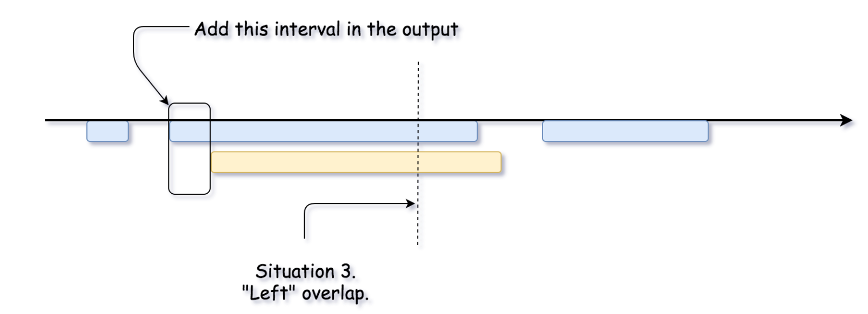
\includegraphics{/Users/harddrive/Desktop/古城算法leetcode.assets/lc1272-3.png?lastModify=1624568391}
\caption{}
\end{figure}

\begin{figure}
\centering
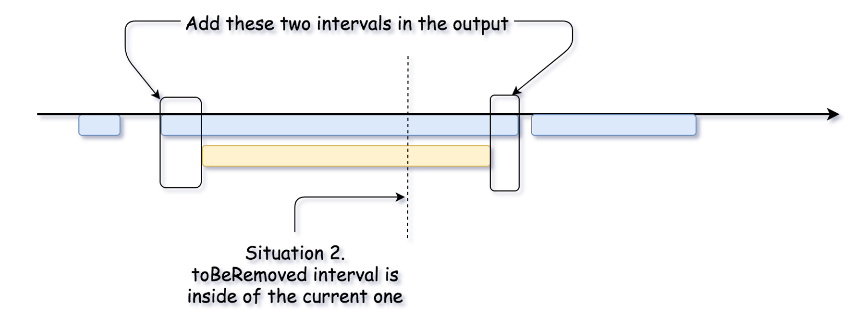
\includegraphics{/Users/harddrive/Desktop/古城算法leetcode.assets/lc1272-2.png?lastModify=1624568391}
\caption{}
\end{figure}

\begin{figure}
\centering
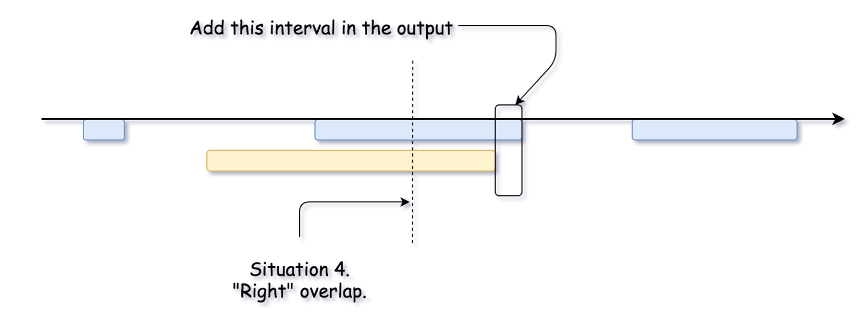
\includegraphics{/Users/harddrive/Desktop/古城算法leetcode.assets/lc1272-1.png?lastModify=1624568391}
\caption{}
\end{figure}

\begin{Shaded}
\begin{Highlighting}[]
\CommentTok{\# VIP 1272 remove interval}
\KeywordTok{def}\NormalTok{ removeInterval(intervals, toBeRemoved):}
\NormalTok{  res }\OperatorTok{=}\NormalTok{ []}
  \ControlFlowTok{for}\NormalTok{ i }\KeywordTok{in}\NormalTok{ intervals:}
    \ControlFlowTok{if}\NormalTok{ i[}\DecValTok{1}\NormalTok{] }\OperatorTok{\textless{}=}\NormalTok{ toBeRemoved[}\DecValTok{0}\NormalTok{] }\KeywordTok{or}\NormalTok{ i[}\DecValTok{0}\NormalTok{] }\OperatorTok{\textgreater{}=}\NormalTok{ toBeRemoved[}\DecValTok{1}\NormalTok{]:  }\CommentTok{\# no overlap}
\NormalTok{      res.append(i)}
    \ControlFlowTok{else}\NormalTok{:}
      \ControlFlowTok{if}\NormalTok{ i[}\DecValTok{0}\NormalTok{] }\OperatorTok{\textless{}}\NormalTok{ toBeRemoved[}\DecValTok{0}\NormalTok{]:  }\CommentTok{\# left end extra remaining}
\NormalTok{        res.append([i[}\DecValTok{0}\NormalTok{], toBeRemoved[}\DecValTok{0}\NormalTok{]])}
      \ControlFlowTok{if}\NormalTok{ i[}\DecValTok{1}\NormalTok{] }\OperatorTok{\textgreater{}}\NormalTok{ toBeRemoved[}\DecValTok{1}\NormalTok{]:  }\CommentTok{\# right end extra remaining}
\NormalTok{        res.append([toBeRemoved[}\DecValTok{1}\NormalTok{], i[}\DecValTok{1}\NormalTok{]])}
  \ControlFlowTok{return}\NormalTok{ res}
\end{Highlighting}
\end{Shaded}

\begin{Shaded}
\begin{Highlighting}[]
\CommentTok{\#https://leetcode.com/problems/the{-}skyline{-}problem/}
\end{Highlighting}
\end{Shaded}

TODO: 1229, 986, 759

\hypertarget{trie-ux5b57ux5178ux6811}{%
\subsection{Trie 字典树}\label{trie-ux5b57ux5178ux6811}}

\begin{Shaded}
\begin{Highlighting}[]
\KeywordTok{class}\NormalTok{ TrieNode:}
    \KeywordTok{def} \FunctionTok{\_\_init\_\_}\NormalTok{(}\VariableTok{self}\NormalTok{):}
        \VariableTok{self}\NormalTok{.children }\OperatorTok{=}\NormalTok{ [}\VariableTok{None}\NormalTok{] }\OperatorTok{*} \DecValTok{26}
        \VariableTok{self}\NormalTok{.is\_word }\OperatorTok{=} \VariableTok{False}
\KeywordTok{class}\NormalTok{ Trie:}

    \KeywordTok{def} \FunctionTok{\_\_init\_\_}\NormalTok{(}\VariableTok{self}\NormalTok{):}
        \CommentTok{"""}
\CommentTok{        Initialize your data structure here.}
\CommentTok{        """}
        \VariableTok{self}\NormalTok{.root }\OperatorTok{=}\NormalTok{ TrieNode()}

    \KeywordTok{def}\NormalTok{ insert(}\VariableTok{self}\NormalTok{, word: }\BuiltInTok{str}\NormalTok{) }\OperatorTok{{-}\textgreater{}} \VariableTok{None}\NormalTok{:}
        \CommentTok{"""}
\CommentTok{        Inserts a word into the trie.}
\CommentTok{        """}
\NormalTok{        node }\OperatorTok{=} \VariableTok{self}\NormalTok{.root}
        \ControlFlowTok{for}\NormalTok{ c }\KeywordTok{in}\NormalTok{ word:}
            \ControlFlowTok{if} \KeywordTok{not}\NormalTok{ node.children[}\BuiltInTok{ord}\NormalTok{(c) }\OperatorTok{{-}} \BuiltInTok{ord}\NormalTok{(}\StringTok{\textquotesingle{}a\textquotesingle{}}\NormalTok{)]:}
\NormalTok{                node.children[}\BuiltInTok{ord}\NormalTok{(c) }\OperatorTok{{-}} \BuiltInTok{ord}\NormalTok{(}\StringTok{\textquotesingle{}a\textquotesingle{}}\NormalTok{)] }\OperatorTok{=}\NormalTok{ TrieNode()}
\NormalTok{            node }\OperatorTok{=}\NormalTok{ node.children[}\BuiltInTok{ord}\NormalTok{(c) }\OperatorTok{{-}} \BuiltInTok{ord}\NormalTok{(}\StringTok{\textquotesingle{}a\textquotesingle{}}\NormalTok{)]}
\NormalTok{        node.is\_word }\OperatorTok{=} \VariableTok{True}

    \KeywordTok{def}\NormalTok{ search(}\VariableTok{self}\NormalTok{, word: }\BuiltInTok{str}\NormalTok{) }\OperatorTok{{-}\textgreater{}} \BuiltInTok{bool}\NormalTok{:}
        \CommentTok{"""}
\CommentTok{        Returns if the word is in the trie.}
\CommentTok{        """}
\NormalTok{        node }\OperatorTok{=} \VariableTok{self}\NormalTok{.root}
        \ControlFlowTok{for}\NormalTok{ c }\KeywordTok{in}\NormalTok{ word:}
            \ControlFlowTok{if} \KeywordTok{not}\NormalTok{ node.children[}\BuiltInTok{ord}\NormalTok{(c) }\OperatorTok{{-}} \BuiltInTok{ord}\NormalTok{(}\StringTok{\textquotesingle{}a\textquotesingle{}}\NormalTok{)]:}
                \ControlFlowTok{return} \VariableTok{False}
\NormalTok{            node }\OperatorTok{=}\NormalTok{ node.children[}\BuiltInTok{ord}\NormalTok{(c) }\OperatorTok{{-}} \BuiltInTok{ord}\NormalTok{(}\StringTok{\textquotesingle{}a\textquotesingle{}}\NormalTok{)]}
        \ControlFlowTok{return}\NormalTok{ node.is\_word}

    \KeywordTok{def}\NormalTok{ startsWith(}\VariableTok{self}\NormalTok{, prefix: }\BuiltInTok{str}\NormalTok{) }\OperatorTok{{-}\textgreater{}} \BuiltInTok{bool}\NormalTok{:}
        \CommentTok{"""}
\CommentTok{        Returns if there is any word in the trie that starts with the given prefix.}
\CommentTok{        """}
\NormalTok{        node }\OperatorTok{=} \VariableTok{self}\NormalTok{.root}
        \ControlFlowTok{for}\NormalTok{ c }\KeywordTok{in}\NormalTok{ prefix:}
            \ControlFlowTok{if} \KeywordTok{not}\NormalTok{ node.children[}\BuiltInTok{ord}\NormalTok{(c) }\OperatorTok{{-}} \BuiltInTok{ord}\NormalTok{(}\StringTok{\textquotesingle{}a\textquotesingle{}}\NormalTok{)]:}
                \ControlFlowTok{return} \VariableTok{False}
\NormalTok{            node }\OperatorTok{=}\NormalTok{ node.children[}\BuiltInTok{ord}\NormalTok{(c) }\OperatorTok{{-}} \BuiltInTok{ord}\NormalTok{(}\StringTok{\textquotesingle{}a\textquotesingle{}}\NormalTok{)]}
        \ControlFlowTok{return} \VariableTok{True}


\CommentTok{\# Your Trie object will be instantiated and called as such:}
\CommentTok{\# obj = Trie()}
\CommentTok{\# obj.insert(word)}
\CommentTok{\# param\_2 = obj.search(word)}
\CommentTok{\# param\_3 = obj.startsWith(prefix)}
\end{Highlighting}
\end{Shaded}

\hypertarget{stack-and-queue}{%
\subsection{Stack and queue}\label{stack-and-queue}}

stack: dequeue interface; queue: LinkedList interface

\begin{Shaded}
\begin{Highlighting}[]
\CommentTok{// haspMap that support addToVal(x) {-}\textgreater{} add x to all values in Map\textless{}int, int\textgreater{}}
\CommentTok{// addToKey(x) {-}\textgreater{} add to all keys in Map}
\KeywordTok{class}\NormalTok{ HashMapAddable}\OperatorTok{\{}
  \DataTypeTok{int}\NormalTok{ keyCount}\OperatorTok{;}
  \DataTypeTok{int}\NormalTok{ valCount}\OperatorTok{;}
  \BuiltInTok{Map}\OperatorTok{\textless{}}\BuiltInTok{Integer}\OperatorTok{,} \BuiltInTok{Integer}\OperatorTok{\textgreater{}}\NormalTok{ map }\OperatorTok{=} \KeywordTok{new} \BuiltInTok{HashMap}\OperatorTok{\textless{}\textgreater{}();}
  \KeywordTok{public} \DataTypeTok{void} \FunctionTok{insert}\OperatorTok{(}\DataTypeTok{int}\OperatorTok{[]}\NormalTok{ nums}\OperatorTok{)\{}
    \DataTypeTok{int}\NormalTok{ insertKey }\OperatorTok{=}\NormalTok{ nums}\OperatorTok{[}\DecValTok{0}\OperatorTok{]} \OperatorTok{{-}}\NormalTok{ keyCountl}\OperatorTok{;}
    \DataTypeTok{int}\NormalTok{ insertVal }\OperatorTok{=}\NormalTok{ nums}\OperatorTok{[}\DecValTok{1}\OperatorTok{]} \OperatorTok{{-}}\NormalTok{ valueCount}\OperatorTok{;}
\NormalTok{    map}\OperatorTok{.}\FunctionTok{put}\OperatorTok{(}\NormalTok{insertKey}\OperatorTok{,}\NormalTok{ insertVal}\OperatorTok{);}
  \OperatorTok{\}}
  \KeywordTok{public} \DataTypeTok{int} \FunctionTok{get}\OperatorTok{(}\DataTypeTok{int}\NormalTok{ key}\OperatorTok{)\{}
    \DataTypeTok{int}\NormalTok{ newKey }\OperatorTok{=}\NormalTok{ key }\OperatorTok{{-}}\NormalTok{ keyCountl}\OperatorTok{;}
    \ControlFlowTok{if} \OperatorTok{(!}\NormalTok{map}\OperatorTok{.}\FunctionTok{containKey}\OperatorTok{(}\NormalTok{newKey}\OperatorTok{))} \ControlFlowTok{return} \OperatorTok{{-}}\DecValTok{1}\OperatorTok{;}
    \DataTypeTok{int}\NormalTok{ newVal }\OperatorTok{=}\NormalTok{ map}\OperatorTok{.}\FunctionTok{get}\OperatorTok{(}\NormalTok{newKey}\OperatorTok{);}
    \ControlFlowTok{return}\NormalTok{ newVal }\OperatorTok{+}\NormalTok{ valCount}\OperatorTok{;}
  \OperatorTok{\}}
  \KeywordTok{public} \DataTypeTok{void} \FunctionTok{addToKey}\OperatorTok{(}\DataTypeTok{int}\NormalTok{ key}\OperatorTok{)\{}\NormalTok{ keyCount }\OperatorTok{+=}\NormalTok{ key}\OperatorTok{;\}}
  \KeywordTok{public} \DataTypeTok{void} \FunctionTok{addToVal}\OperatorTok{(}\DataTypeTok{int}\NormalTok{ val}\OperatorTok{)\{}\NormalTok{ valCount }\OperatorTok{+=}\NormalTok{ key}\OperatorTok{;\}}
\OperatorTok{\}}
\end{Highlighting}
\end{Shaded}

\hypertarget{disjoint-setunion-find}{%
\subsection{Disjoint set/union find}\label{disjoint-setunion-find}}

Tree like structure that only cares about parent (group).

Used in dynamic connectivity problem.

\begin{Shaded}
\begin{Highlighting}[]
\CommentTok{\# easy}
\KeywordTok{class}\NormalTok{ DisjointSet():}
    \KeywordTok{def} \FunctionTok{\_\_init\_\_}\NormalTok{(}\VariableTok{self}\NormalTok{, n):}
        \VariableTok{self}\NormalTok{.parent }\OperatorTok{=}\NormalTok{ [i }\ControlFlowTok{for}\NormalTok{ i }\KeywordTok{in} \BuiltInTok{range}\NormalTok{(n)]}
    \KeywordTok{def}\NormalTok{ find(x):}
        \ControlFlowTok{if} \VariableTok{self}\NormalTok{.parent[x] }\OperatorTok{!=}\NormalTok{ x:}
            \CommentTok{\# simple path compression}
            \VariableTok{self}\NormalTok{.parent[x] }\OperatorTok{=} \VariableTok{self}\NormalTok{.find(}\VariableTok{self}\NormalTok{.parent[x])}
        \ControlFlowTok{return}\NormalTok{ x}
   	\KeywordTok{def}\NormalTok{ union(x, y):   }
\NormalTok{        parent[}\VariableTok{self}\NormalTok{.find(x)] }\OperatorTok{=} \VariableTok{self}\NormalTok{.find(y)}

\KeywordTok{class}\NormalTok{ DisjointSet():}
    \KeywordTok{def} \FunctionTok{\_\_init\_\_}\NormalTok{(}\VariableTok{self}\NormalTok{, n):}
        \VariableTok{self}\NormalTok{.parent }\OperatorTok{=}\NormalTok{ [i }\ControlFlowTok{for}\NormalTok{ i }\KeywordTok{in} \BuiltInTok{range}\NormalTok{(n)]}
        \VariableTok{self}\NormalTok{.size }\OperatorTok{=}\NormalTok{ [}\DecValTok{1}\NormalTok{] }\OperatorTok{*}\NormalTok{ n  }
    \KeywordTok{def}\NormalTok{ find(x):}
        \ControlFlowTok{if} \VariableTok{self}\NormalTok{.parent[x] }\OperatorTok{!=}\NormalTok{ x:}
            \CommentTok{\# simple path compression}
            \VariableTok{self}\NormalTok{.parent[x] }\OperatorTok{=} \VariableTok{self}\NormalTok{.find(}\VariableTok{self}\NormalTok{.parent[x])}
        \ControlFlowTok{return}\NormalTok{ x}
   	\KeywordTok{def}\NormalTok{ union(x, y):   }
        \CommentTok{\# weight optimized: to reduce the number of parent changing in path compression, always merge small subtree into large one}
\NormalTok{        parent[}\VariableTok{self}\NormalTok{.find(x)] }\OperatorTok{=} \VariableTok{self}\NormalTok{.find(y)}
\NormalTok{        rootx , rooty }\OperatorTok{=} \VariableTok{self}\NormalTok{.find(x), }\VariableTok{self}\NormalTok{.find(y)}
        \ControlFlowTok{if}\NormalTok{ rootx }\OperatorTok{==}\NormalTok{ rooty: }\ControlFlowTok{return}
        \ControlFlowTok{if} \VariableTok{self}\NormalTok{.size[rooty] }\OperatorTok{\textless{}=} \VariableTok{self}\NormalTok{.size[rootx]:}
            \VariableTok{self}\NormalTok{.parent[rooty] }\OperatorTok{=}\NormalTok{ rootx}
            \VariableTok{self}\NormalTok{.size[rootx] }\OperatorTok{+=} \VariableTok{self}\NormalTok{.size[rooty]}
        \ControlFlowTok{else}\NormalTok{:}
            \VariableTok{self}\NormalTok{.parent[rootx] }\OperatorTok{=}\NormalTok{ rooty}
            \VariableTok{self}\NormalTok{.size[rooty] }\OperatorTok{+=} \VariableTok{self}\NormalTok{.size[rootx]}
\end{Highlighting}
\end{Shaded}

Each Find and Union has O(log* n) runtime, where n is the size of union
find. Log* is iterative logarithm, which is close to amortized O(1).

\href{https://leetcode.com/problems/number-of-provinces}{Number of
Provinces}

\begin{Shaded}
\begin{Highlighting}[]
\CommentTok{\# Amortized O(n\^{}2). Each element in isConnected call union/find.}
\KeywordTok{class}\NormalTok{ Solution:}
    \KeywordTok{def}\NormalTok{ findCircleNum(}\VariableTok{self}\NormalTok{, isConnected: List[List[}\BuiltInTok{int}\NormalTok{]]) }\OperatorTok{{-}\textgreater{}} \BuiltInTok{int}\NormalTok{:}
\NormalTok{        n }\OperatorTok{=} \BuiltInTok{len}\NormalTok{(isConnected)}
\NormalTok{        dsu }\OperatorTok{=}\NormalTok{ DSU(n)}
        \ControlFlowTok{for}\NormalTok{ i }\KeywordTok{in} \BuiltInTok{range}\NormalTok{(n):}
            \ControlFlowTok{for}\NormalTok{ j }\KeywordTok{in} \BuiltInTok{range}\NormalTok{(i):}
                \ControlFlowTok{if}\NormalTok{ i }\OperatorTok{==}\NormalTok{ j }\KeywordTok{or}\NormalTok{ isConnected[i][j] }\OperatorTok{==} \DecValTok{0}\NormalTok{: }\ControlFlowTok{continue}
\NormalTok{                dsu.union(i, j)}
\NormalTok{        res }\OperatorTok{=} \DecValTok{0}
        \ControlFlowTok{for}\NormalTok{ i }\KeywordTok{in} \BuiltInTok{range}\NormalTok{(n): }
            \ControlFlowTok{if}\NormalTok{ dsu.find(i) }\OperatorTok{==}\NormalTok{ i: }
\NormalTok{                res }\OperatorTok{+=} \DecValTok{1}
        \ControlFlowTok{return}\NormalTok{ res}

\KeywordTok{class}\NormalTok{ DSU: }
    \KeywordTok{def} \FunctionTok{\_\_init\_\_}\NormalTok{(}\VariableTok{self}\NormalTok{, n):}
        \VariableTok{self}\NormalTok{.p }\OperatorTok{=}\NormalTok{ [i }\ControlFlowTok{for}\NormalTok{ i }\KeywordTok{in} \BuiltInTok{range}\NormalTok{(n)]}
    \KeywordTok{def}\NormalTok{ find(}\VariableTok{self}\NormalTok{, x):}
        \ControlFlowTok{if} \VariableTok{self}\NormalTok{.p[x] }\OperatorTok{!=}\NormalTok{ x:}
            \VariableTok{self}\NormalTok{.p[x] }\OperatorTok{=} \VariableTok{self}\NormalTok{.find(}\VariableTok{self}\NormalTok{.p[x])}
        \ControlFlowTok{return} \VariableTok{self}\NormalTok{.p[x]}
    \KeywordTok{def}\NormalTok{ union(}\VariableTok{self}\NormalTok{,x , y):}
        \VariableTok{self}\NormalTok{.p[}\VariableTok{self}\NormalTok{.find(x)] }\OperatorTok{=} \VariableTok{self}\NormalTok{.find(y)}

\end{Highlighting}
\end{Shaded}

\hypertarget{number-of-islands}{%
\subsection{Number of Islands}\label{number-of-islands}}

\hypertarget{dfs-bfs-union-find-path-to-secribe-shape-tarjans-algo-distributed-processing}{%
\subsubsection{DFS; BFS; Union Find; Path to secribe shape; Tarjan's
Algo; Distributed
processing}\label{dfs-bfs-union-find-path-to-secribe-shape-tarjans-algo-distributed-processing}}

\begin{Shaded}
\begin{Highlighting}[]
\CommentTok{\# number of island}
\CommentTok{\# DFS }
\NormalTok{dirs }\OperatorTok{=}\NormalTok{ [[}\DecValTok{0}\NormalTok{,}\DecValTok{1}\NormalTok{], [}\DecValTok{0}\NormalTok{,}\OperatorTok{{-}}\DecValTok{1}\NormalTok{], [}\DecValTok{1}\NormalTok{,}\DecValTok{0}\NormalTok{], [}\OperatorTok{{-}}\DecValTok{1}\NormalTok{,}\DecValTok{0}\NormalTok{]]}
\KeywordTok{def}\NormalTok{ dfs(x, y):}
  \ControlFlowTok{if}\NormalTok{ x }\OperatorTok{\textless{}} \DecValTok{0} \KeywordTok{or}\NormalTok{ y }\OperatorTok{\textless{}} \DecValTok{0} \KeywordTok{or}\NormalTok{ x }\OperatorTok{\textgreater{}=} \BuiltInTok{len}\NormalTok{(grid) }\KeywordTok{or}\NormalTok{ y }\OperatorTok{\textgreater{}} \BuiltInTok{len}\NormalTok{(grid[}\DecValTok{0}\NormalTok{]) }\KeywordTok{or}\NormalTok{ grid[x][y] }\OperatorTok{!=} \StringTok{\textquotesingle{}1\textquotesingle{}}\NormalTok{: }\ControlFlowTok{return}
\NormalTok{  grid[x][y] }\OperatorTok{=} \StringTok{\textquotesingle{}0\textquotesingle{}}
  \ControlFlowTok{for} \BuiltInTok{dir} \KeywordTok{in}\NormalTok{ dirs:}
\NormalTok{    dfs(x}\OperatorTok{+}\BuiltInTok{dir}\NormalTok{[}\DecValTok{0}\NormalTok{], y}\OperatorTok{+}\BuiltInTok{dir}\NormalTok{[}\DecValTok{1}\NormalTok{])}
\CommentTok{\# DFS iterative}
\KeywordTok{def}\NormalTok{ dfs(x, y):}
  \ControlFlowTok{if}\NormalTok{ x }\OperatorTok{\textless{}} \DecValTok{0} \KeywordTok{or}\NormalTok{ y }\OperatorTok{\textless{}} \DecValTok{0} \KeywordTok{or}\NormalTok{ x }\OperatorTok{\textgreater{}=} \BuiltInTok{len}\NormalTok{(grid) }\KeywordTok{or}\NormalTok{ y }\OperatorTok{\textgreater{}} \BuiltInTok{len}\NormalTok{(grid[}\DecValTok{0}\NormalTok{]) }\KeywordTok{or}\NormalTok{ grid[x][y] }\OperatorTok{!=} \StringTok{\textquotesingle{}1\textquotesingle{}}\NormalTok{: }\ControlFlowTok{return}
\NormalTok{  stack }\OperatorTok{=}\NormalTok{ [(x, y)]}
  \ControlFlowTok{while}\NormalTok{ stack:}
\NormalTok{    i, j }\OperatorTok{=}\NormalTok{ stack.pop()}
    \ControlFlowTok{if}\NormalTok{ i }\OperatorTok{\textless{}} \DecValTok{0} \KeywordTok{or}\NormalTok{ j }\OperatorTok{\textless{}} \DecValTok{0} \KeywordTok{or}\NormalTok{ i }\OperatorTok{\textgreater{}=} \BuiltInTok{len}\NormalTok{(grid) }\KeywordTok{or}\NormalTok{ j }\OperatorTok{\textgreater{}} \BuiltInTok{len}\NormalTok{(grid[}\DecValTok{0}\NormalTok{]) }\KeywordTok{or}\NormalTok{ grid[i][j] }\OperatorTok{!=} \StringTok{\textquotesingle{}1\textquotesingle{}}\NormalTok{: }\ControlFlowTok{continue}
\NormalTok{    grid[i][j] }\OperatorTok{=} \StringTok{\textquotesingle{}0\textquotesingle{}}
    \ControlFlowTok{for} \BuiltInTok{dir} \KeywordTok{in}\NormalTok{ dirs:}
\NormalTok{      q.append((i}\OperatorTok{+}\BuiltInTok{dir}\NormalTok{[}\DecValTok{0}\NormalTok{], j}\OperatorTok{+}\BuiltInTok{dir}\NormalTok{[}\DecValTok{1}\NormalTok{]))}
\CommentTok{\# BFS}
\KeywordTok{def}\NormalTok{ bfs(x, y):}
  \ControlFlowTok{if}\NormalTok{ x }\OperatorTok{\textless{}} \DecValTok{0} \KeywordTok{or}\NormalTok{ y }\OperatorTok{\textless{}} \DecValTok{0} \KeywordTok{or}\NormalTok{ x }\OperatorTok{\textgreater{}=} \BuiltInTok{len}\NormalTok{(grid) }\KeywordTok{or}\NormalTok{ y }\OperatorTok{\textgreater{}} \BuiltInTok{len}\NormalTok{(grid[}\DecValTok{0}\NormalTok{]) }\KeywordTok{or}\NormalTok{ grid[x][y] }\OperatorTok{!=} \StringTok{\textquotesingle{}1\textquotesingle{}}\NormalTok{: }\ControlFlowTok{return}
\NormalTok{  q }\OperatorTok{=}\NormalTok{ deque([(x,y)])}
  \ControlFlowTok{while}\NormalTok{ q: }
\NormalTok{    i, j }\OperatorTok{=}\NormalTok{ q.popleft()}
    \ControlFlowTok{if}\NormalTok{ i }\OperatorTok{\textless{}} \DecValTok{0} \KeywordTok{or}\NormalTok{ j }\OperatorTok{\textless{}} \DecValTok{0} \KeywordTok{or}\NormalTok{ i }\OperatorTok{\textgreater{}=} \BuiltInTok{len}\NormalTok{(grid) }\KeywordTok{or}\NormalTok{ j }\OperatorTok{\textgreater{}} \BuiltInTok{len}\NormalTok{(grid[}\DecValTok{0}\NormalTok{]) }\KeywordTok{or}\NormalTok{ grid[i][j] }\OperatorTok{!=} \StringTok{\textquotesingle{}1\textquotesingle{}}\NormalTok{: }\ControlFlowTok{continue}
\NormalTok{    grid[i][j] }\OperatorTok{=} \StringTok{\textquotesingle{}0\textquotesingle{}}
    \ControlFlowTok{for} \BuiltInTok{dir} \KeywordTok{in}\NormalTok{ dirs:}
\NormalTok{      q.append((i}\OperatorTok{+}\BuiltInTok{dir}\NormalTok{[}\DecValTok{0}\NormalTok{], j}\OperatorTok{+}\BuiltInTok{dir}\NormalTok{[}\DecValTok{1}\NormalTok{]))}
\KeywordTok{def}\NormalTok{ numIslands(grid: List[List[}\BuiltInTok{str}\NormalTok{]]) }\OperatorTok{{-}\textgreater{}} \BuiltInTok{int}\NormalTok{:}
\NormalTok{  cnt }\OperatorTok{=} \DecValTok{0}
  \ControlFlowTok{for}\NormalTok{ i }\KeywordTok{in} \BuiltInTok{range}\NormalTok{(}\BuiltInTok{len}\NormalTok{(grid)):}
    \ControlFlowTok{for}\NormalTok{ j }\KeywordTok{in} \BuiltInTok{range}\NormalTok{(}\BuiltInTok{len}\NormalTok{(grid[}\DecValTok{0}\NormalTok{])):}
      \ControlFlowTok{if}\NormalTok{ grid[i][j] }\OperatorTok{==} \StringTok{\textquotesingle{}1\textquotesingle{}}\NormalTok{:}
\NormalTok{        dfs(i, j)  }\OperatorTok{/}\NormalTok{ bfs(i, j)}
\NormalTok{      	cnt }\OperatorTok{+=} \DecValTok{1}
  \ControlFlowTok{return}\NormalTok{ cnt}
\end{Highlighting}
\end{Shaded}

\hypertarget{sort}{%
\subsection{Sort}\label{sort}}

\begin{Shaded}
\begin{Highlighting}[]
\CommentTok{\# quicksort, best case T(n) = O(n) + 2 O(n/2) + ...= nlgn}
\CommentTok{\# worst case T(n) = T(n) + T(n{-}1) + ... = n\^{}2}
\KeywordTok{def}\NormalTok{ quickSort(arr, low, high):}
    \ControlFlowTok{if}\NormalTok{ low }\OperatorTok{\textgreater{}=}\NormalTok{ high: }\ControlFlowTok{return}
\NormalTok{    pv }\OperatorTok{=}\NormalTok{ partition(arr, low, high)}
\NormalTok{    quickSort(arr, low, pv}\OperatorTok{{-}}\DecValTok{1}\NormalTok{)}
\NormalTok{    quickSort(arr, pv}\OperatorTok{+}\DecValTok{1}\NormalTok{, high)}

\KeywordTok{def}\NormalTok{ partition(arr, low, high):}
\NormalTok{    wall }\OperatorTok{=}\NormalTok{ low}
\NormalTok{    pivot }\OperatorTok{=}\NormalTok{ arr[high]}
    \ControlFlowTok{for}\NormalTok{ i }\KeywordTok{in} \BuiltInTok{range}\NormalTok{(low, high):}
        \CommentTok{\# make sure left of wall is nonstrictly smaller than pivot}
        \ControlFlowTok{if}\NormalTok{ arr[i] }\OperatorTok{\textless{}=}\NormalTok{ pivot:}
\NormalTok{            arr[wall], arr[i] }\OperatorTok{=}\NormalTok{ arr[i], arr[wall]}
\NormalTok{            wall }\OperatorTok{+=} \DecValTok{1}
\NormalTok{    arr[high], arr[wall] }\OperatorTok{=}\NormalTok{ arr[wall], arr[high]}
\end{Highlighting}
\end{Shaded}

\hypertarget{divide-and-conquer}{%
\subsection{Divide and conquer}\label{divide-and-conquer}}

\begin{Shaded}
\begin{Highlighting}[]
\CommentTok{\# inversion pairs: }
\CommentTok{\# find all the pairs st. nums[i] \textgreater{} num[j] and i \textless{} j}
\CommentTok{\# a large number that has a small index}
\CommentTok{\# 3 1 2 {-}\textgreater{} 31, 32 }
\CommentTok{\# 8 4 2 1 {-}\textgreater{} 84, 82, 81, 42, 41, 21}
\CommentTok{\# start with merge sort, we count the number of such pairs in the merging step}
\KeywordTok{def}\NormalTok{ mergesortCount(arr, l, r):}
\NormalTok{	cnt }\OperatorTok{=} \DecValTok{0}
  \ControlFlowTok{if}\NormalTok{ l }\OperatorTok{\textless{}}\NormalTok{ r:}
\NormalTok{    m }\OperatorTok{=}\NormalTok{ (l }\OperatorTok{+}\NormalTok{ r) }\OperatorTok{//} \DecValTok{2}
\NormalTok{    count }\OperatorTok{+=}\NormalTok{ mergesortCount(arr, l, m)}
\NormalTok{    count }\OperatorTok{+=}\NormalTok{ mergesortCount(arr, m}\OperatorTok{+}\DecValTok{1}\NormalTok{, r)}
\NormalTok{    count }\OperatorTok{+=}\NormalTok{ mergeCount(arr, l, m, r)}
\KeywordTok{def}\NormalTok{ mergeCount(arr, l, m, r):}
\NormalTok{  left }\OperatorTok{=}\NormalTok{ arr[l:m}\OperatorTok{+}\DecValTok{1}\NormalTok{]}
\NormalTok{  right }\OperatorTok{=}\NormalTok{ arr[m}\OperatorTok{+}\DecValTok{1}\NormalTok{:r}\OperatorTok{+}\DecValTok{1}\NormalTok{]}
\NormalTok{  i }\OperatorTok{=}\NormalTok{ j }\OperatorTok{=}\NormalTok{ k }\OperatorTok{=} \DecValTok{0}
\NormalTok{ 	swap }\OperatorTok{=} \DecValTok{0}
  \ControlFlowTok{while}\NormalTok{ i }\OperatorTok{\textless{}} \BuiltInTok{len}\NormalTok{(left) }\KeywordTok{and}\NormalTok{ j }\OperatorTok{\textless{}} \BuiltInTok{len}\NormalTok{(right):}
    \ControlFlowTok{if}\NormalTok{ left[i] }\OperatorTok{\textless{}=}\NormalTok{ right[j]:}
\NormalTok{      arr[k] }\OperatorTok{=}\NormalTok{ left[i]}
\NormalTok{      k }\OperatorTok{+=} \DecValTok{1}\OperatorTok{;}\NormalTok{ i }\OperatorTok{+=} \DecValTok{1}
    \ControlFlowTok{else}\NormalTok{:}
\NormalTok{      arr[k] }\OperatorTok{=}\NormalTok{ right[j]}
\NormalTok{      k }\OperatorTok{+=} \DecValTok{1}\OperatorTok{;}\NormalTok{ j }\OperatorTok{+=} \DecValTok{1}
\NormalTok{      swap }\OperatorTok{+=}\NormalTok{ m }\OperatorTok{{-}}\NormalTok{ (l }\OperatorTok{+}\NormalTok{ r) }\OperatorTok{+} \DecValTok{1}
  \ControlFlowTok{return}\NormalTok{ swap}
\CommentTok{\# master theorem}
\NormalTok{T(n) }\OperatorTok{=}\NormalTok{ a T(n}\OperatorTok{/}\NormalTok{b) }\OperatorTok{+}\NormalTok{ O(n}\OperatorTok{\^{}}\NormalTok{c)}
\NormalTok{c}\OperatorTok{\^{}}\NormalTok{crit }\OperatorTok{=}\NormalTok{ log\_b(a)}
\FloatTok{1.}\NormalTok{ c }\OperatorTok{\textless{}}\NormalTok{ c\_crit, leaf}\OperatorTok{{-}}\NormalTok{heavy }\OperatorTok{=\textgreater{}}\NormalTok{ O(n}\OperatorTok{\^{}}\NormalTok{c\_crit)}
\FloatTok{2.}\NormalTok{ c }\OperatorTok{=}\NormalTok{ c\_crit, comparable }\OperatorTok{{-}\textgreater{}}\NormalTok{ rewrite f(n) part into O(n}\OperatorTok{\^{}}\NormalTok{c log}\OperatorTok{\^{}}\NormalTok{k n) }\OperatorTok{=\textgreater{}}\NormalTok{ O(n}\OperatorTok{\^{}}\NormalTok{crit log}\OperatorTok{\^{}}\NormalTok{(k}\OperatorTok{+}\DecValTok{1}\NormalTok{) n)}
\FloatTok{3.}\NormalTok{ c }\OperatorTok{\textgreater{}}\NormalTok{ c\_crit, root\_heavy }\OperatorTok{=\textgreater{}}\NormalTok{ O(n}\OperatorTok{\^{}}\NormalTok{c)}

\FloatTok{1.}\NormalTok{T(n) }\OperatorTok{=} \DecValTok{8}\NormalTok{T(n}\OperatorTok{/}\DecValTok{2}\NormalTok{) }\OperatorTok{+} \DecValTok{1000}\NormalTok{n}\OperatorTok{\^{}}\DecValTok{2} \OperatorTok{=\textgreater{}}\NormalTok{ O(n}\OperatorTok{\^{}}\DecValTok{3}\NormalTok{)}
\FloatTok{2.}\NormalTok{T(n) }\OperatorTok{=} \DecValTok{2}\NormalTok{(T}\OperatorTok{/}\DecValTok{2}\NormalTok{) }\OperatorTok{+} \DecValTok{10}\NormalTok{n }\OperatorTok{=\textgreater{}}\NormalTok{ O(nlogn)}
\FloatTok{3.}\NormalTok{T(n) }\OperatorTok{=} \DecValTok{2}\NormalTok{(T}\OperatorTok{/}\DecValTok{2}\NormalTok{) }\OperatorTok{+}\NormalTok{ n}\OperatorTok{\^{}}\DecValTok{2} \OperatorTok{=\textgreater{}}\NormalTok{ O(n}\OperatorTok{\^{}}\DecValTok{2}\NormalTok{)}
\end{Highlighting}
\end{Shaded}

\hypertarget{serialize-and-deserialize}{%
\subsection{Serialize and Deserialize}\label{serialize-and-deserialize}}

\begin{Shaded}
\begin{Highlighting}[]
\CommentTok{\# 297 }
\CommentTok{\# Use preorder traversal to do the serialization step}
\CommentTok{\# The resulting string has the form}
\CommentTok{\# | Root | Left Subtree | Right Subtree |}
\CommentTok{\# Use recursion to deserialize that string}

\KeywordTok{class}\NormalTok{ Codec:}

    \KeywordTok{def}\NormalTok{ serialize(}\VariableTok{self}\NormalTok{, root):}
        \CommentTok{"""Encodes a tree to a single string.}
\CommentTok{        }
\CommentTok{        :type root: TreeNode}
\CommentTok{        :rtype: str}
\CommentTok{        """}
        \CommentTok{\# preorder traversal}
        \ControlFlowTok{if} \KeywordTok{not}\NormalTok{ root: }\ControlFlowTok{return} \StringTok{"\#"}
        \ControlFlowTok{return} \BuiltInTok{str}\NormalTok{(root.val) }\OperatorTok{+} \StringTok{","} \OperatorTok{+} \VariableTok{self}\NormalTok{.serialize(root.left) }\OperatorTok{+} \StringTok{","} \OperatorTok{+} \VariableTok{self}\NormalTok{.serialize(root.right)}


    \KeywordTok{def}\NormalTok{ deserialize(}\VariableTok{self}\NormalTok{, data):}
        \CommentTok{"""Decodes your encoded data to tree.}
\CommentTok{        }
\CommentTok{        :type data: str}
\CommentTok{        :rtype: TreeNode}
\CommentTok{        """}
        \KeywordTok{def}\NormalTok{ helper(data):}
\NormalTok{            s }\OperatorTok{=}\NormalTok{ data.popleft()}
            \ControlFlowTok{if}\NormalTok{ s }\OperatorTok{==} \StringTok{"\#"}\NormalTok{: }\ControlFlowTok{return} \VariableTok{None}
\NormalTok{            root }\OperatorTok{=}\NormalTok{ TreeNode(}\BuiltInTok{int}\NormalTok{(s))}
\NormalTok{            root.left }\OperatorTok{=}\NormalTok{ helper(data)}
\NormalTok{            root.right }\OperatorTok{=}\NormalTok{ helper(data)}
            \ControlFlowTok{return}\NormalTok{ root}
        \ControlFlowTok{return}\NormalTok{ helper(collections.deque(data.split(}\StringTok{\textquotesingle{},\textquotesingle{}}\NormalTok{)))}
\end{Highlighting}
\end{Shaded}

\hypertarget{ux4fe1ux606fux4f20ux9012}{%
\subsection{信息传递}\label{ux4fe1ux606fux4f20ux9012}}

backtracking is similar to DFS, one kind of brute force. (ex Nqueen
problem). Usually its helper function returns void (no early quit in
order to brute force all); and stores information in nonlocal variables.

257

\hypertarget{ignored-hard}{%
\subsection{Ignored Hard}\label{ignored-hard}}

352 Data Stream as Disjoint Intervals
\href{https://www.youtube.com/watch?v=ihf8JjQdta0\&t=1221s}{扫描线}

\href{https://leetcode.com/problems/maximum-frequency-stack}{Maximum
Frequency Stack}
\href{https://www.youtube.com/watch?v=cV3SpacBh3M\&t=11s}{Stack}

\hypertarget{ignored-vip}{%
\subsection{Ignored VIP}\label{ignored-vip}}

\href{https://leetcode.com/problems/meeting-scheduler}{ Meeting
Scheduler}

\href{https://leetcode.com/problems/employee-free-time}{Employee Free
Time}

\end{document}
